% Options for packages loaded elsewhere
\PassOptionsToPackage{unicode}{hyperref}
\PassOptionsToPackage{hyphens}{url}
\PassOptionsToPackage{dvipsnames,svgnames,x11names}{xcolor}
%
\documentclass[
]{article}
\usepackage{amsmath,amssymb}
\usepackage{iftex}
\ifPDFTeX
  \usepackage[T1]{fontenc}
  \usepackage[utf8]{inputenc}
  \usepackage{textcomp} % provide euro and other symbols
\else % if luatex or xetex
  \usepackage{unicode-math} % this also loads fontspec
  \defaultfontfeatures{Scale=MatchLowercase}
  \defaultfontfeatures[\rmfamily]{Ligatures=TeX,Scale=1}
\fi
\usepackage{lmodern}
\ifPDFTeX\else
  % xetex/luatex font selection
\fi
% Use upquote if available, for straight quotes in verbatim environments
\IfFileExists{upquote.sty}{\usepackage{upquote}}{}
\IfFileExists{microtype.sty}{% use microtype if available
  \usepackage[]{microtype}
  \UseMicrotypeSet[protrusion]{basicmath} % disable protrusion for tt fonts
}{}
\makeatletter
\@ifundefined{KOMAClassName}{% if non-KOMA class
  \IfFileExists{parskip.sty}{%
    \usepackage{parskip}
  }{% else
    \setlength{\parindent}{0pt}
    \setlength{\parskip}{6pt plus 2pt minus 1pt}}
}{% if KOMA class
  \KOMAoptions{parskip=half}}
\makeatother
\usepackage{xcolor}
\usepackage[margin=1in]{geometry}
\usepackage{color}
\usepackage{fancyvrb}
\newcommand{\VerbBar}{|}
\newcommand{\VERB}{\Verb[commandchars=\\\{\}]}
\DefineVerbatimEnvironment{Highlighting}{Verbatim}{commandchars=\\\{\}}
% Add ',fontsize=\small' for more characters per line
\usepackage{framed}
\definecolor{shadecolor}{RGB}{248,248,248}
\newenvironment{Shaded}{\begin{snugshade}}{\end{snugshade}}
\newcommand{\AlertTok}[1]{\textcolor[rgb]{0.94,0.16,0.16}{#1}}
\newcommand{\AnnotationTok}[1]{\textcolor[rgb]{0.56,0.35,0.01}{\textbf{\textit{#1}}}}
\newcommand{\AttributeTok}[1]{\textcolor[rgb]{0.13,0.29,0.53}{#1}}
\newcommand{\BaseNTok}[1]{\textcolor[rgb]{0.00,0.00,0.81}{#1}}
\newcommand{\BuiltInTok}[1]{#1}
\newcommand{\CharTok}[1]{\textcolor[rgb]{0.31,0.60,0.02}{#1}}
\newcommand{\CommentTok}[1]{\textcolor[rgb]{0.56,0.35,0.01}{\textit{#1}}}
\newcommand{\CommentVarTok}[1]{\textcolor[rgb]{0.56,0.35,0.01}{\textbf{\textit{#1}}}}
\newcommand{\ConstantTok}[1]{\textcolor[rgb]{0.56,0.35,0.01}{#1}}
\newcommand{\ControlFlowTok}[1]{\textcolor[rgb]{0.13,0.29,0.53}{\textbf{#1}}}
\newcommand{\DataTypeTok}[1]{\textcolor[rgb]{0.13,0.29,0.53}{#1}}
\newcommand{\DecValTok}[1]{\textcolor[rgb]{0.00,0.00,0.81}{#1}}
\newcommand{\DocumentationTok}[1]{\textcolor[rgb]{0.56,0.35,0.01}{\textbf{\textit{#1}}}}
\newcommand{\ErrorTok}[1]{\textcolor[rgb]{0.64,0.00,0.00}{\textbf{#1}}}
\newcommand{\ExtensionTok}[1]{#1}
\newcommand{\FloatTok}[1]{\textcolor[rgb]{0.00,0.00,0.81}{#1}}
\newcommand{\FunctionTok}[1]{\textcolor[rgb]{0.13,0.29,0.53}{\textbf{#1}}}
\newcommand{\ImportTok}[1]{#1}
\newcommand{\InformationTok}[1]{\textcolor[rgb]{0.56,0.35,0.01}{\textbf{\textit{#1}}}}
\newcommand{\KeywordTok}[1]{\textcolor[rgb]{0.13,0.29,0.53}{\textbf{#1}}}
\newcommand{\NormalTok}[1]{#1}
\newcommand{\OperatorTok}[1]{\textcolor[rgb]{0.81,0.36,0.00}{\textbf{#1}}}
\newcommand{\OtherTok}[1]{\textcolor[rgb]{0.56,0.35,0.01}{#1}}
\newcommand{\PreprocessorTok}[1]{\textcolor[rgb]{0.56,0.35,0.01}{\textit{#1}}}
\newcommand{\RegionMarkerTok}[1]{#1}
\newcommand{\SpecialCharTok}[1]{\textcolor[rgb]{0.81,0.36,0.00}{\textbf{#1}}}
\newcommand{\SpecialStringTok}[1]{\textcolor[rgb]{0.31,0.60,0.02}{#1}}
\newcommand{\StringTok}[1]{\textcolor[rgb]{0.31,0.60,0.02}{#1}}
\newcommand{\VariableTok}[1]{\textcolor[rgb]{0.00,0.00,0.00}{#1}}
\newcommand{\VerbatimStringTok}[1]{\textcolor[rgb]{0.31,0.60,0.02}{#1}}
\newcommand{\WarningTok}[1]{\textcolor[rgb]{0.56,0.35,0.01}{\textbf{\textit{#1}}}}
\usepackage{graphicx}
\makeatletter
\def\maxwidth{\ifdim\Gin@nat@width>\linewidth\linewidth\else\Gin@nat@width\fi}
\def\maxheight{\ifdim\Gin@nat@height>\textheight\textheight\else\Gin@nat@height\fi}
\makeatother
% Scale images if necessary, so that they will not overflow the page
% margins by default, and it is still possible to overwrite the defaults
% using explicit options in \includegraphics[width, height, ...]{}
\setkeys{Gin}{width=\maxwidth,height=\maxheight,keepaspectratio}
% Set default figure placement to htbp
\makeatletter
\def\fps@figure{htbp}
\makeatother
\setlength{\emergencystretch}{3em} % prevent overfull lines
\providecommand{\tightlist}{%
  \setlength{\itemsep}{0pt}\setlength{\parskip}{0pt}}
\setcounter{secnumdepth}{-\maxdimen} % remove section numbering
% definitions for citeproc citations
\NewDocumentCommand\citeproctext{}{}
\NewDocumentCommand\citeproc{mm}{%
  \begingroup\def\citeproctext{#2}\cite{#1}\endgroup}
\makeatletter
 % allow citations to break across lines
 \let\@cite@ofmt\@firstofone
 % avoid brackets around text for \cite:
 \def\@biblabel#1{}
 \def\@cite#1#2{{#1\if@tempswa , #2\fi}}
\makeatother
\newlength{\cslhangindent}
\setlength{\cslhangindent}{1.5em}
\newlength{\csllabelwidth}
\setlength{\csllabelwidth}{3em}
\newenvironment{CSLReferences}[2] % #1 hanging-indent, #2 entry-spacing
 {\begin{list}{}{%
  \setlength{\itemindent}{0pt}
  \setlength{\leftmargin}{0pt}
  \setlength{\parsep}{0pt}
  % turn on hanging indent if param 1 is 1
  \ifodd #1
   \setlength{\leftmargin}{\cslhangindent}
   \setlength{\itemindent}{-1\cslhangindent}
  \fi
  % set entry spacing
  \setlength{\itemsep}{#2\baselineskip}}}
 {\end{list}}
\usepackage{calc}
\newcommand{\CSLBlock}[1]{\hfill\break\parbox[t]{\linewidth}{\strut\ignorespaces#1\strut}}
\newcommand{\CSLLeftMargin}[1]{\parbox[t]{\csllabelwidth}{\strut#1\strut}}
\newcommand{\CSLRightInline}[1]{\parbox[t]{\linewidth - \csllabelwidth}{\strut#1\strut}}
\newcommand{\CSLIndent}[1]{\hspace{\cslhangindent}#1}
\ifLuaTeX
  \usepackage{selnolig}  % disable illegal ligatures
\fi
\usepackage{bookmark}
\IfFileExists{xurl.sty}{\usepackage{xurl}}{} % add URL line breaks if available
\urlstyle{same}
\hypersetup{
  pdftitle={A hands-on tutorial on R and RStudio},
  pdfauthor={Tiago A. Marques},
  colorlinks=true,
  linkcolor={Maroon},
  filecolor={Maroon},
  citecolor={Blue},
  urlcolor={blue},
  pdfcreator={LaTeX via pandoc}}

\title{A hands-on tutorial on R and RStudio}
\usepackage{etoolbox}
\makeatletter
\providecommand{\subtitle}[1]{% add subtitle to \maketitle
  \apptocmd{\@title}{\par {\large #1 \par}}{}{}
}
\makeatother
\subtitle{A tutorial that might get used for lots of stuff}
\author{Tiago A. Marques}
\date{22 October 2024}

\begin{document}
\maketitle

{
\hypersetup{linkcolor=}
\setcounter{tocdepth}{3}
\tableofcontents
}
\begin{center}\rule{0.5\linewidth}{0.5pt}\end{center}

\begin{center}\rule{0.5\linewidth}{0.5pt}\end{center}

\newpage

\section{Before you start}\label{before-you-start}

\subsection{Where is this tutorial?}\label{where-is-this-tutorial}

You might be reading this document as a pdf, a word or an html. This is
in itself a dynamic report in RMarkdown (see more details about dynamic
reports below). The .Rmd which, after compilation, creates them all, is
available in the github repository located at:

\url{https://github.com/TiagoAMarques/AnIntro2RTutorial}

\subsection{Tutorial versions}\label{tutorial-versions}

This .Rmd was last compiled on 2024-10-22 19:06:25.647311. The latest
version of this tutorial is always available at the github repository
above.

\subsection{Tips for non-UK native system
users}\label{tips-for-non-uk-native-system-users}

You should avoid file names with anything other than small
english-language letters as characters, including Latin characters like
``é'', ``ã'', ``ô'' or ``ç'', say. Also avoid spaces in file names. In
short, make them short and easily readable, as possible. Also, you
should be aware that some directories names can cause issues. If you are
a user with those characters in the name, and you are working via a user
with your name, then this applies to you. Finaly, be careful about some
directories not having necessarily the name (for the system) that
Windows shows you to have (examples for PT users: ``Utilizador'' vs
``User'' and ``desktop'' vs ``Ambiente de trabalho'').

\section{Introduction}\label{introduction}

This tutorial was created as a gentle introduction to the
\href{https://www.r-project.org/}{R} environment via the
\href{https://www.rstudio.com/}{RStudio} interface to R. While it could
be a general introduction to R, the primary objective of this document
is to serve as a ``hands-on-tutorial'' for courses delivered by me
(TAM). I use it for both Ecologia Numérica and Modelação Ecológica, at
FCUL, as well as for some other courses. It does not assume any previous
knowledge about R, but some basic logic and programming notions would be
desirable.

To facilitate the interaction with R we leverage on
\href{https://www.rstudio.com/}{RStudio}, a piece of software which
allows users to have at a click's distance many useful features in R. In
the following sections of the tutorial you will be guided through a
first session of R via RStudio.

The tutorial is intended to follow a brief presentation about R and
RStudio, their interaction and capabilities (``Quick introduction to R
and RStudio.pptx'', also in this git repository). Since September 2023
there is also a shinny-new version of that presentation on RPubs:
\url{https://rpubs.com/talomarques/RRStudioRMarkdown}

This tutorial assumes that R and RStudio have been previously installed
in the computer you are using. The latest version of both software
packages is recommended. Both are free and open source.

Disclaimer: in this document I copy paste freely from other documents
that I have written. Therefore, if you have read these words elsewhere
by me, though luck. I claim the right to plagiarize myself here!

\section{Preliminaries about R}\label{preliminaries-about-r}

There is an extensive community revolving around R, and abundant
courses, tutorials, books, blogs, list servers, etc, are freely
available online.

R might seem frightening at first, but even monsters can make something
look more pleasant if you look from the right angle. It is all a matter
of perspective :) So I will use the help of some monsters here to
convince you that this is the right thing to do!

The amazing images in this document are all by Allison Horst, Artwork by
'@'allison\_horst, and I recommend you visit Allison's github repository
filled up with amazing stats and maths illustrations
(\url{https://github.com/allisonhorst/stats-illustrations}), including
so many amazing resources to make R look less frightening. To be honest,
this section is actually also an homage to Allison's outstanding work.

\begin{figure}
\centering

\includegraphics{extfiles/monsteRs.jpg}
\caption{Illustrating R Monsters: Artwork by '@'allison\_horst}
\end{figure}

And it is not just about stats. If you do not understand how to find the
derivative of a function after looking at Artwork by Allison Horst and
her amazing visualization series on the topic, take it as a sign: just
give it up, as I suspect you will never will!

\begin{figure}
\centering
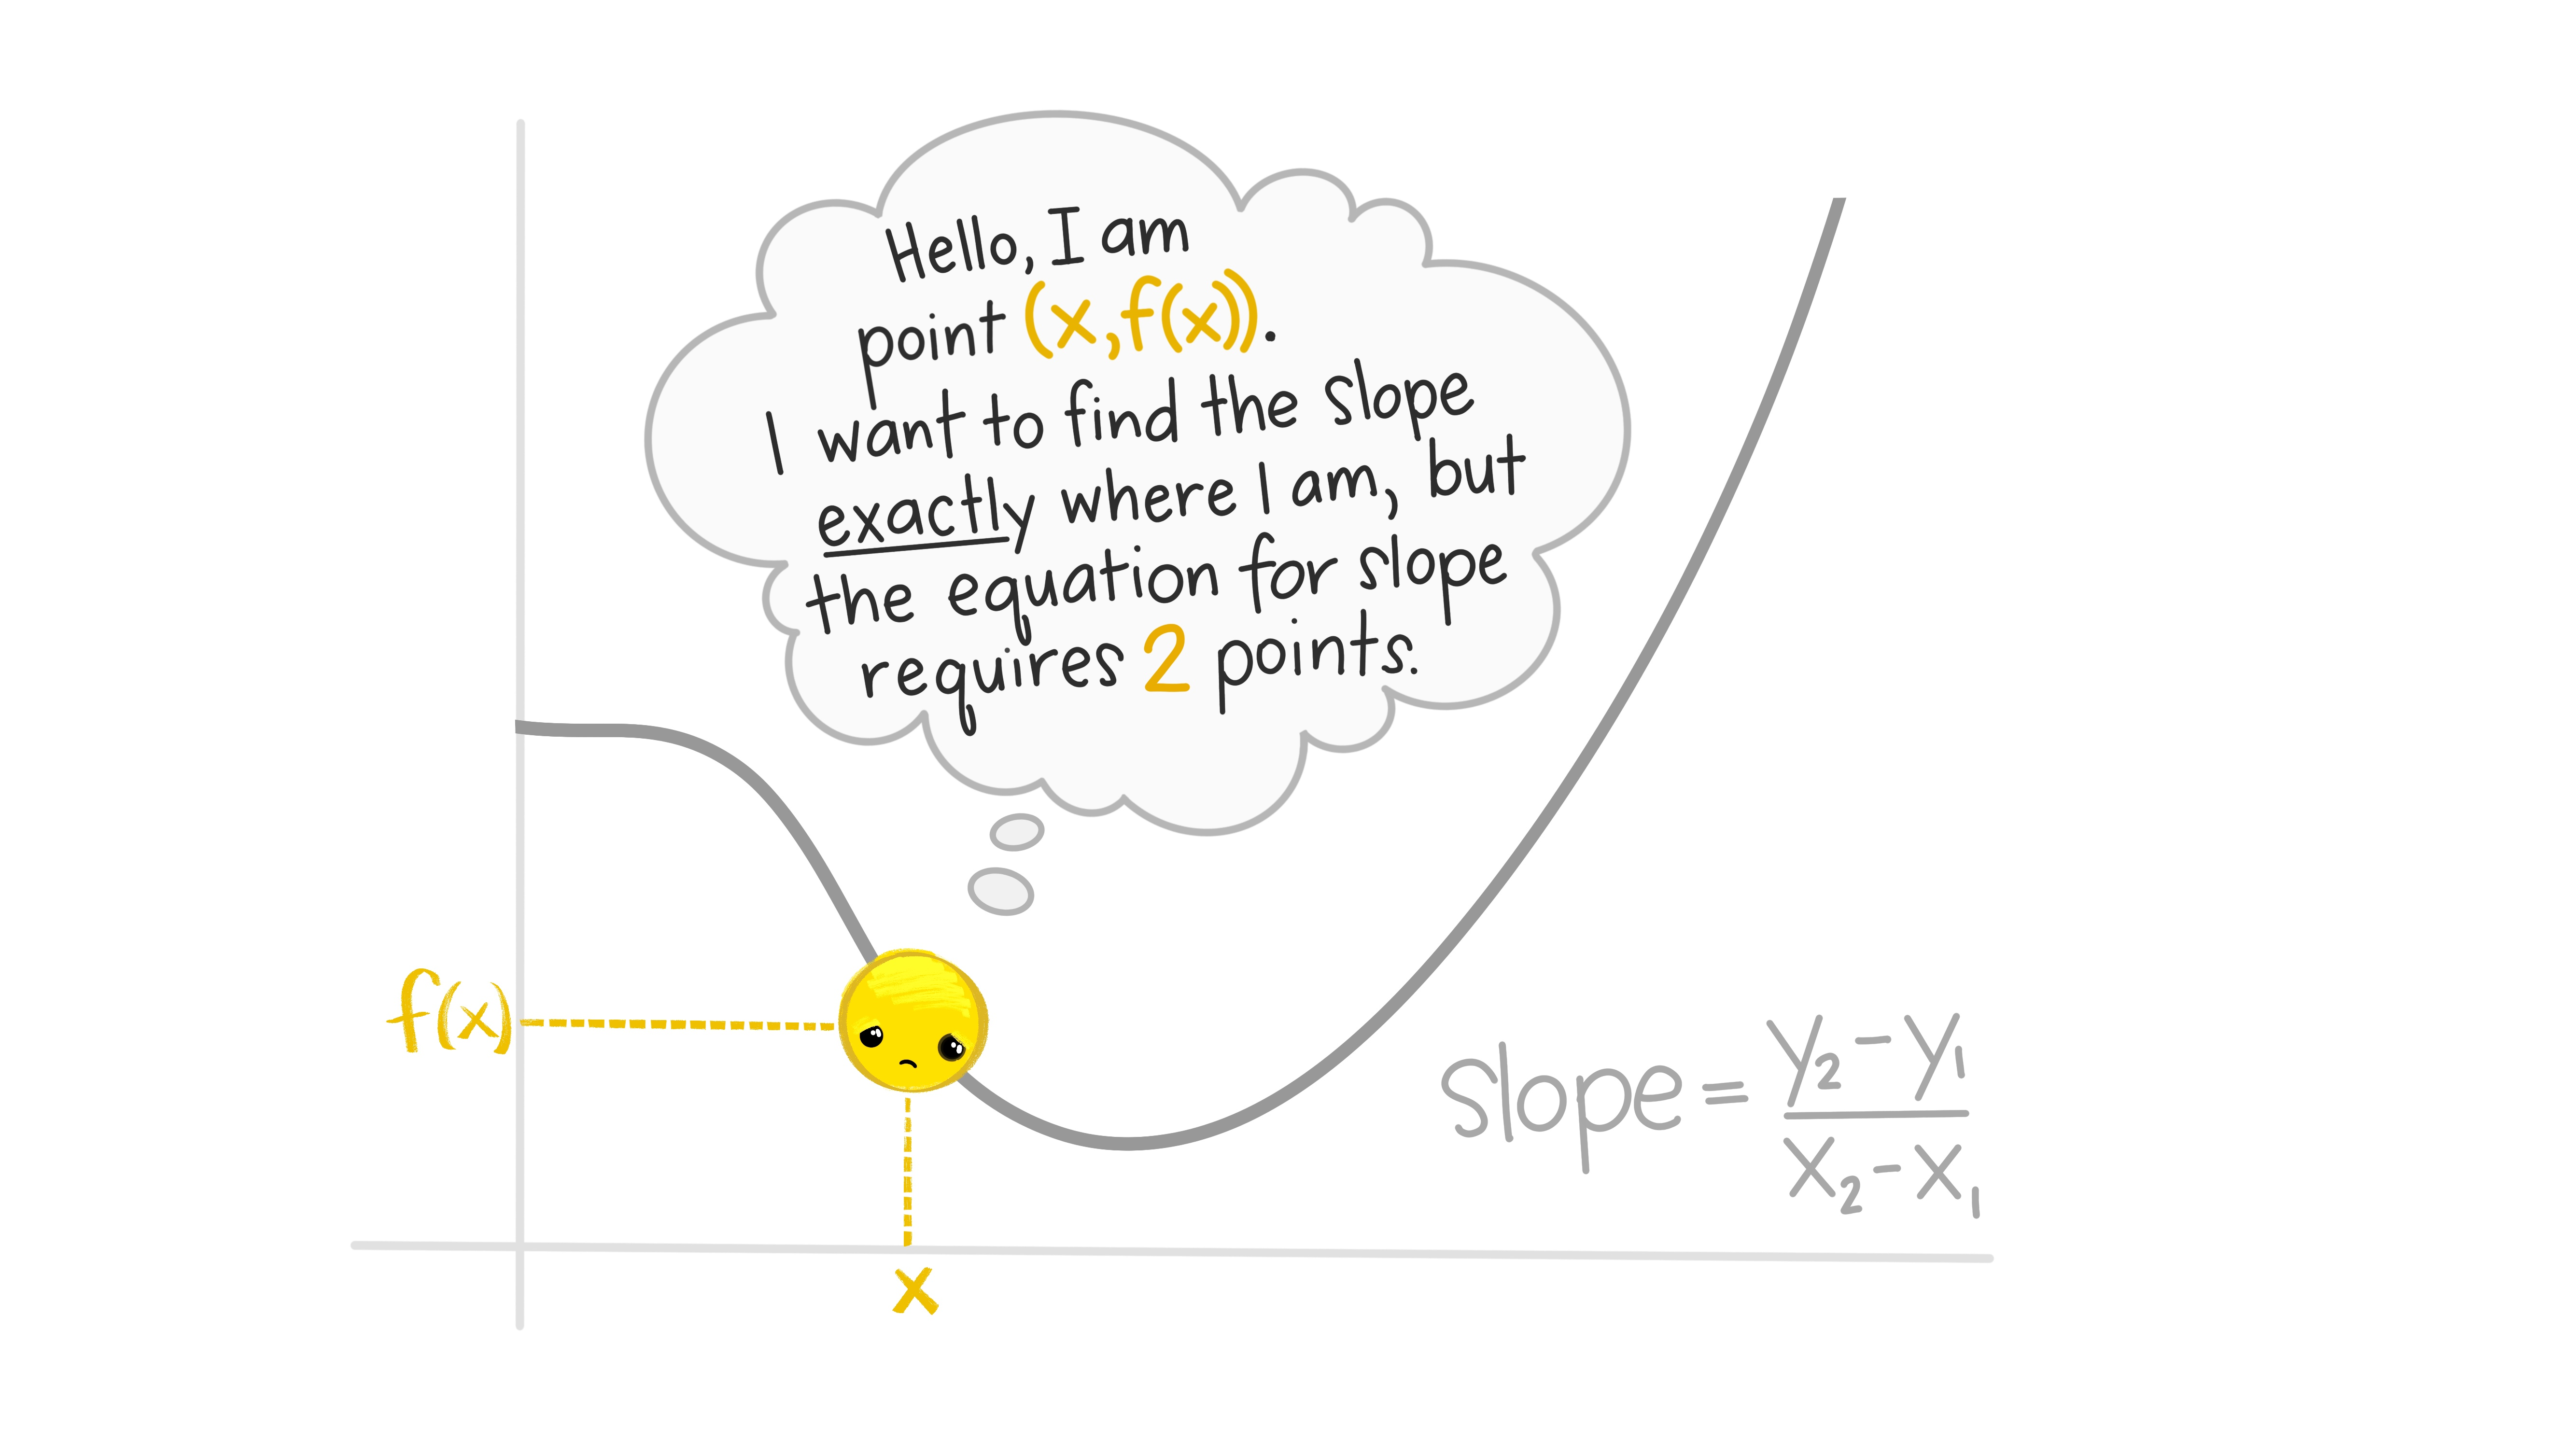
\includegraphics{extfiles/derivative_1.jpg}
\caption{Illustrating a Derivative: Artwork by '@'allison\_horst}
\end{figure}

Nowadays learning R by example is easy to do, with so many free online
resources available to do so.

\begin{figure}
\centering

\includegraphics{extfiles/monster_support.jpg}
\caption{Illustrating learning R online: Artwork by '@'allison\_horst}
\end{figure}

I recommend that you do it via the RStudio environment, since it
provides an integrated environment to integrate with all R things. And
there are many! And if you do so, I can guarantee that in no time you
will be having fRun.

\begin{figure}
\centering

\includegraphics{extfiles/r_first_then.png}
\caption{Illustrating having funR: Artwork by '@'allison\_horst}
\end{figure}

The advantages of mastering R are priceless, but the learning curve can
be daunting at first.

\begin{figure}
\centering
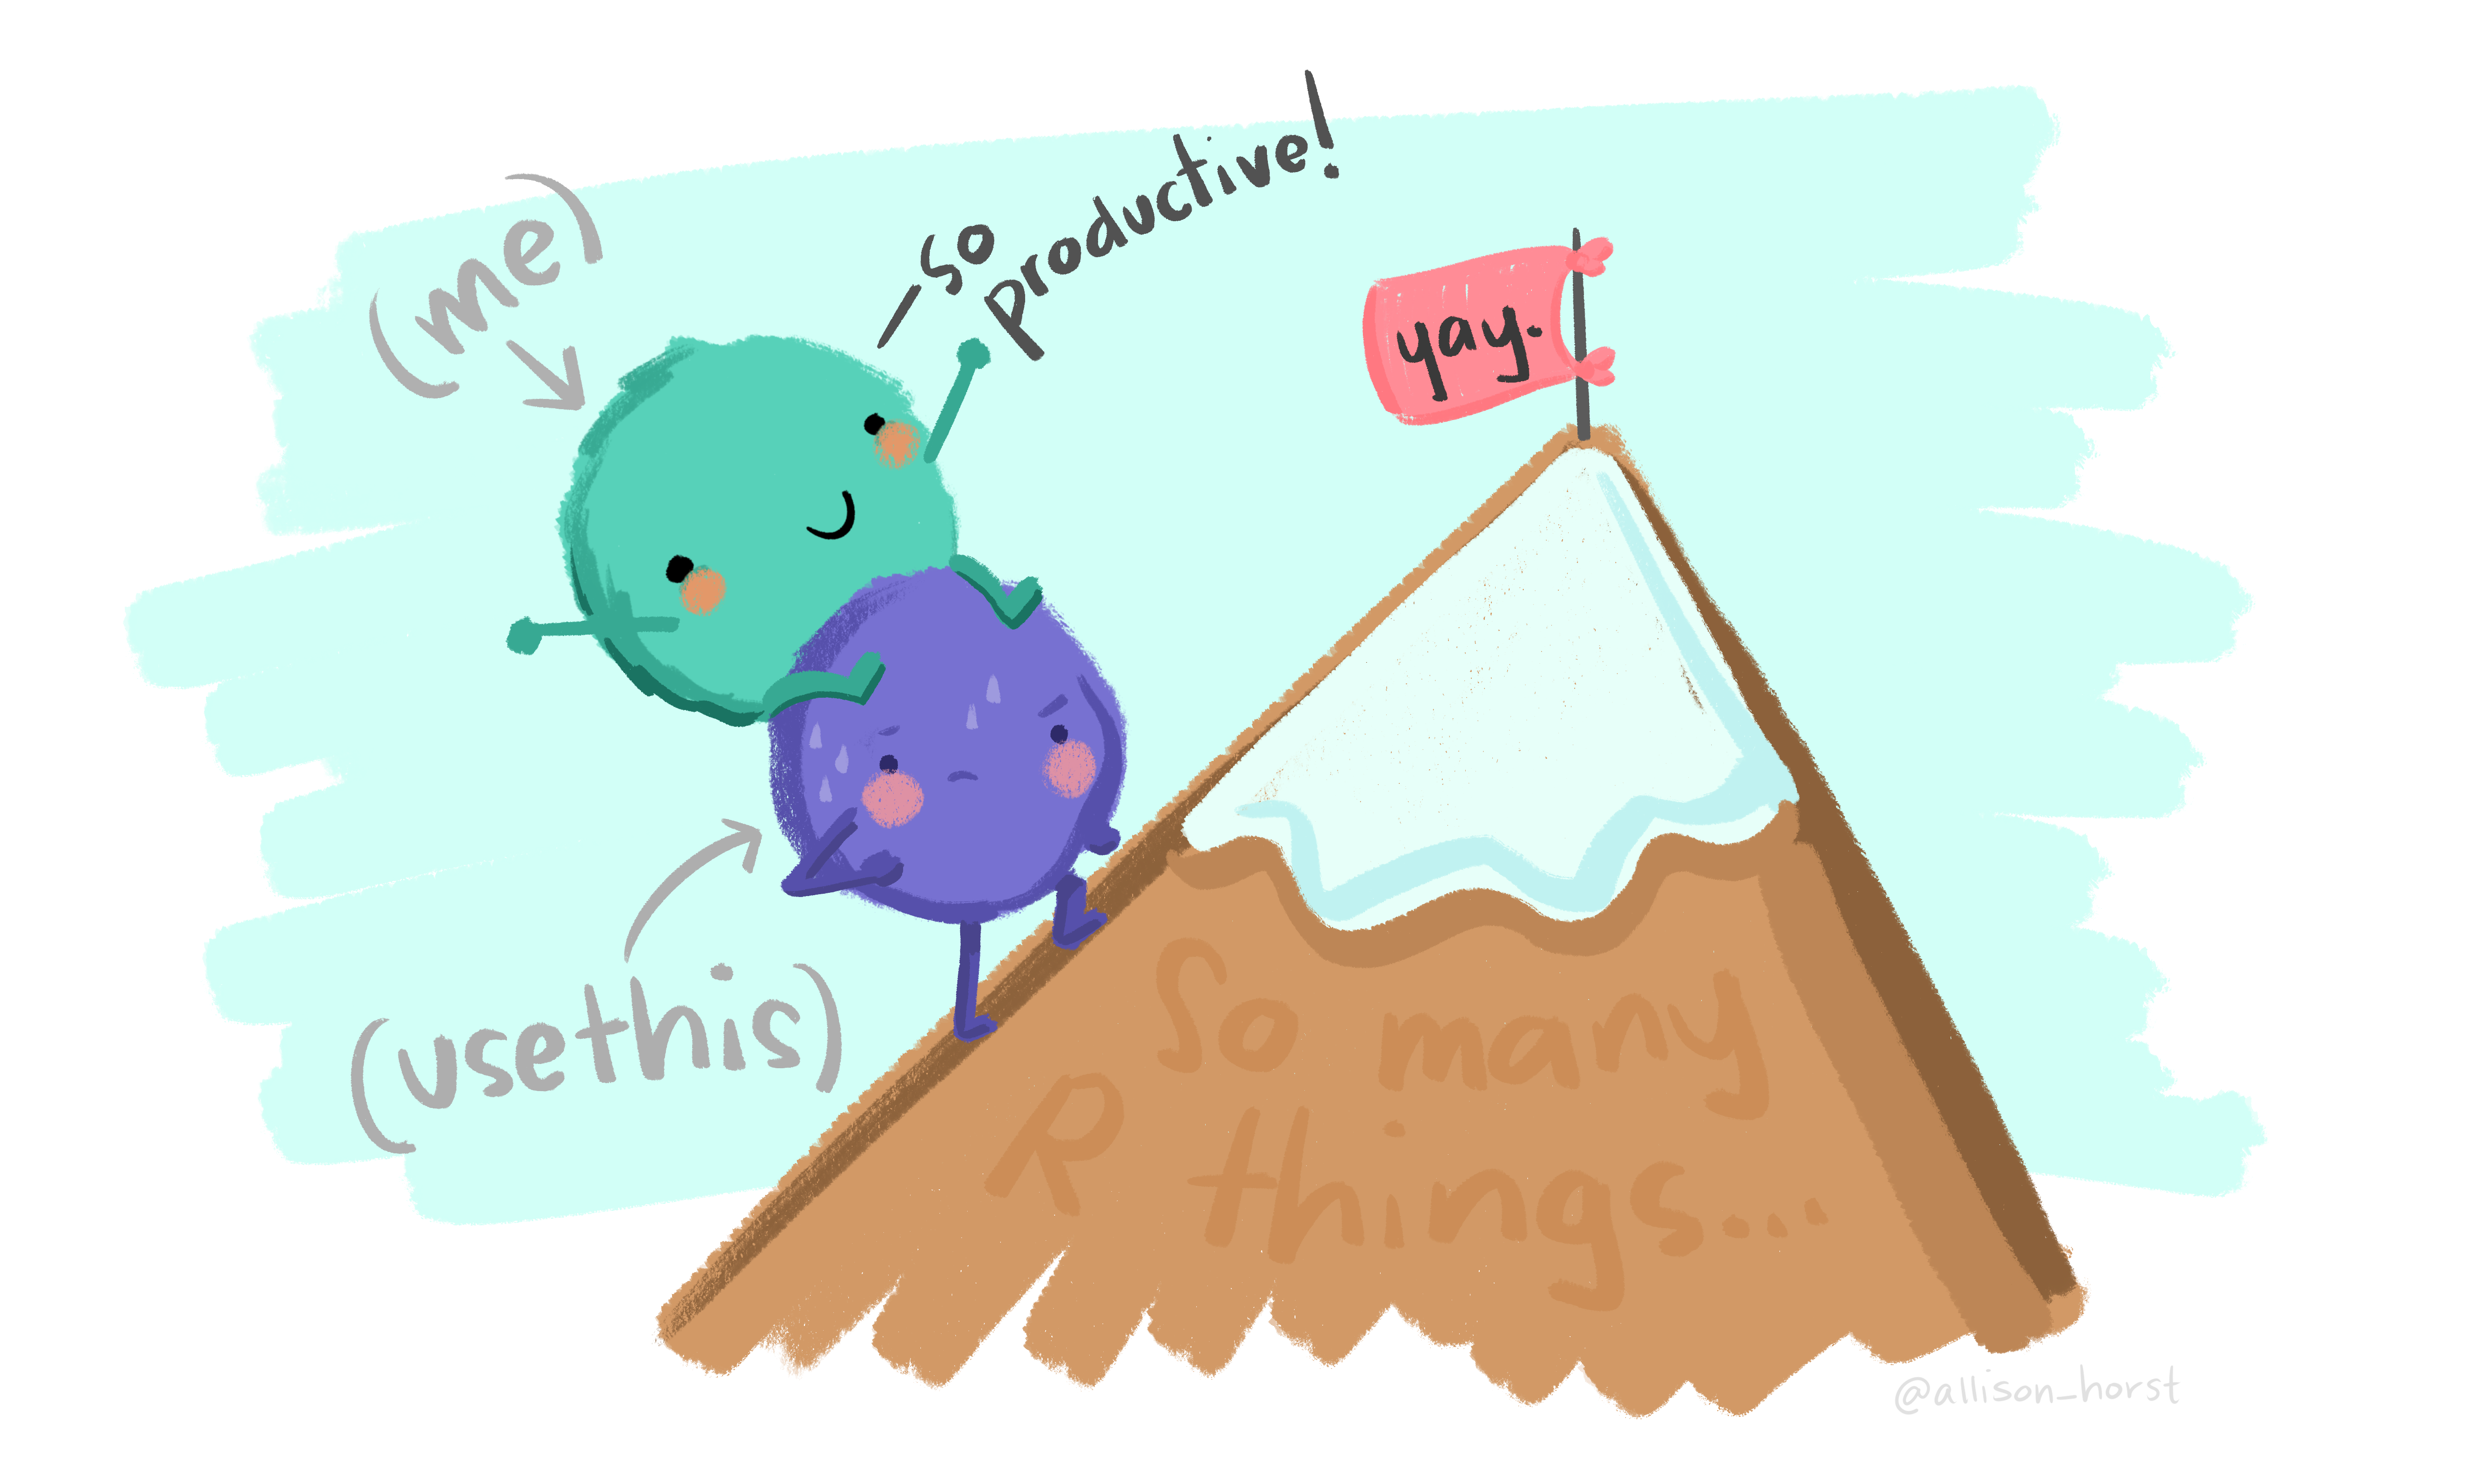
\includegraphics{extfiles/usethis.png}
\caption{Illustrating R's learning curve: Artwork by '@'allison\_horst}
\end{figure}

This document is written in RMarkdown, a tool that allows you to build
dynamic reports based on R code, providing integrated documents that
contain all that is required for a given project, from reading the data
in to final results and discussion, passing through all the analysis and
results. If you want a gentle introduction to RMarkdown using a hands on
tutorial based on a versatile template that will do many of the things
you will need to get started, look for no more, there is also one here:

\url{https://github.com/TiagoAMarques/RMarkdownTemplate}

Go out and explore, little grasshopper. You will conquer many great
things if you do. You will become a code giant one day. But never
forget, you need to be thankful to an entire community, and you are
standing on the shoulders of giants!

\begin{figure}
\centering
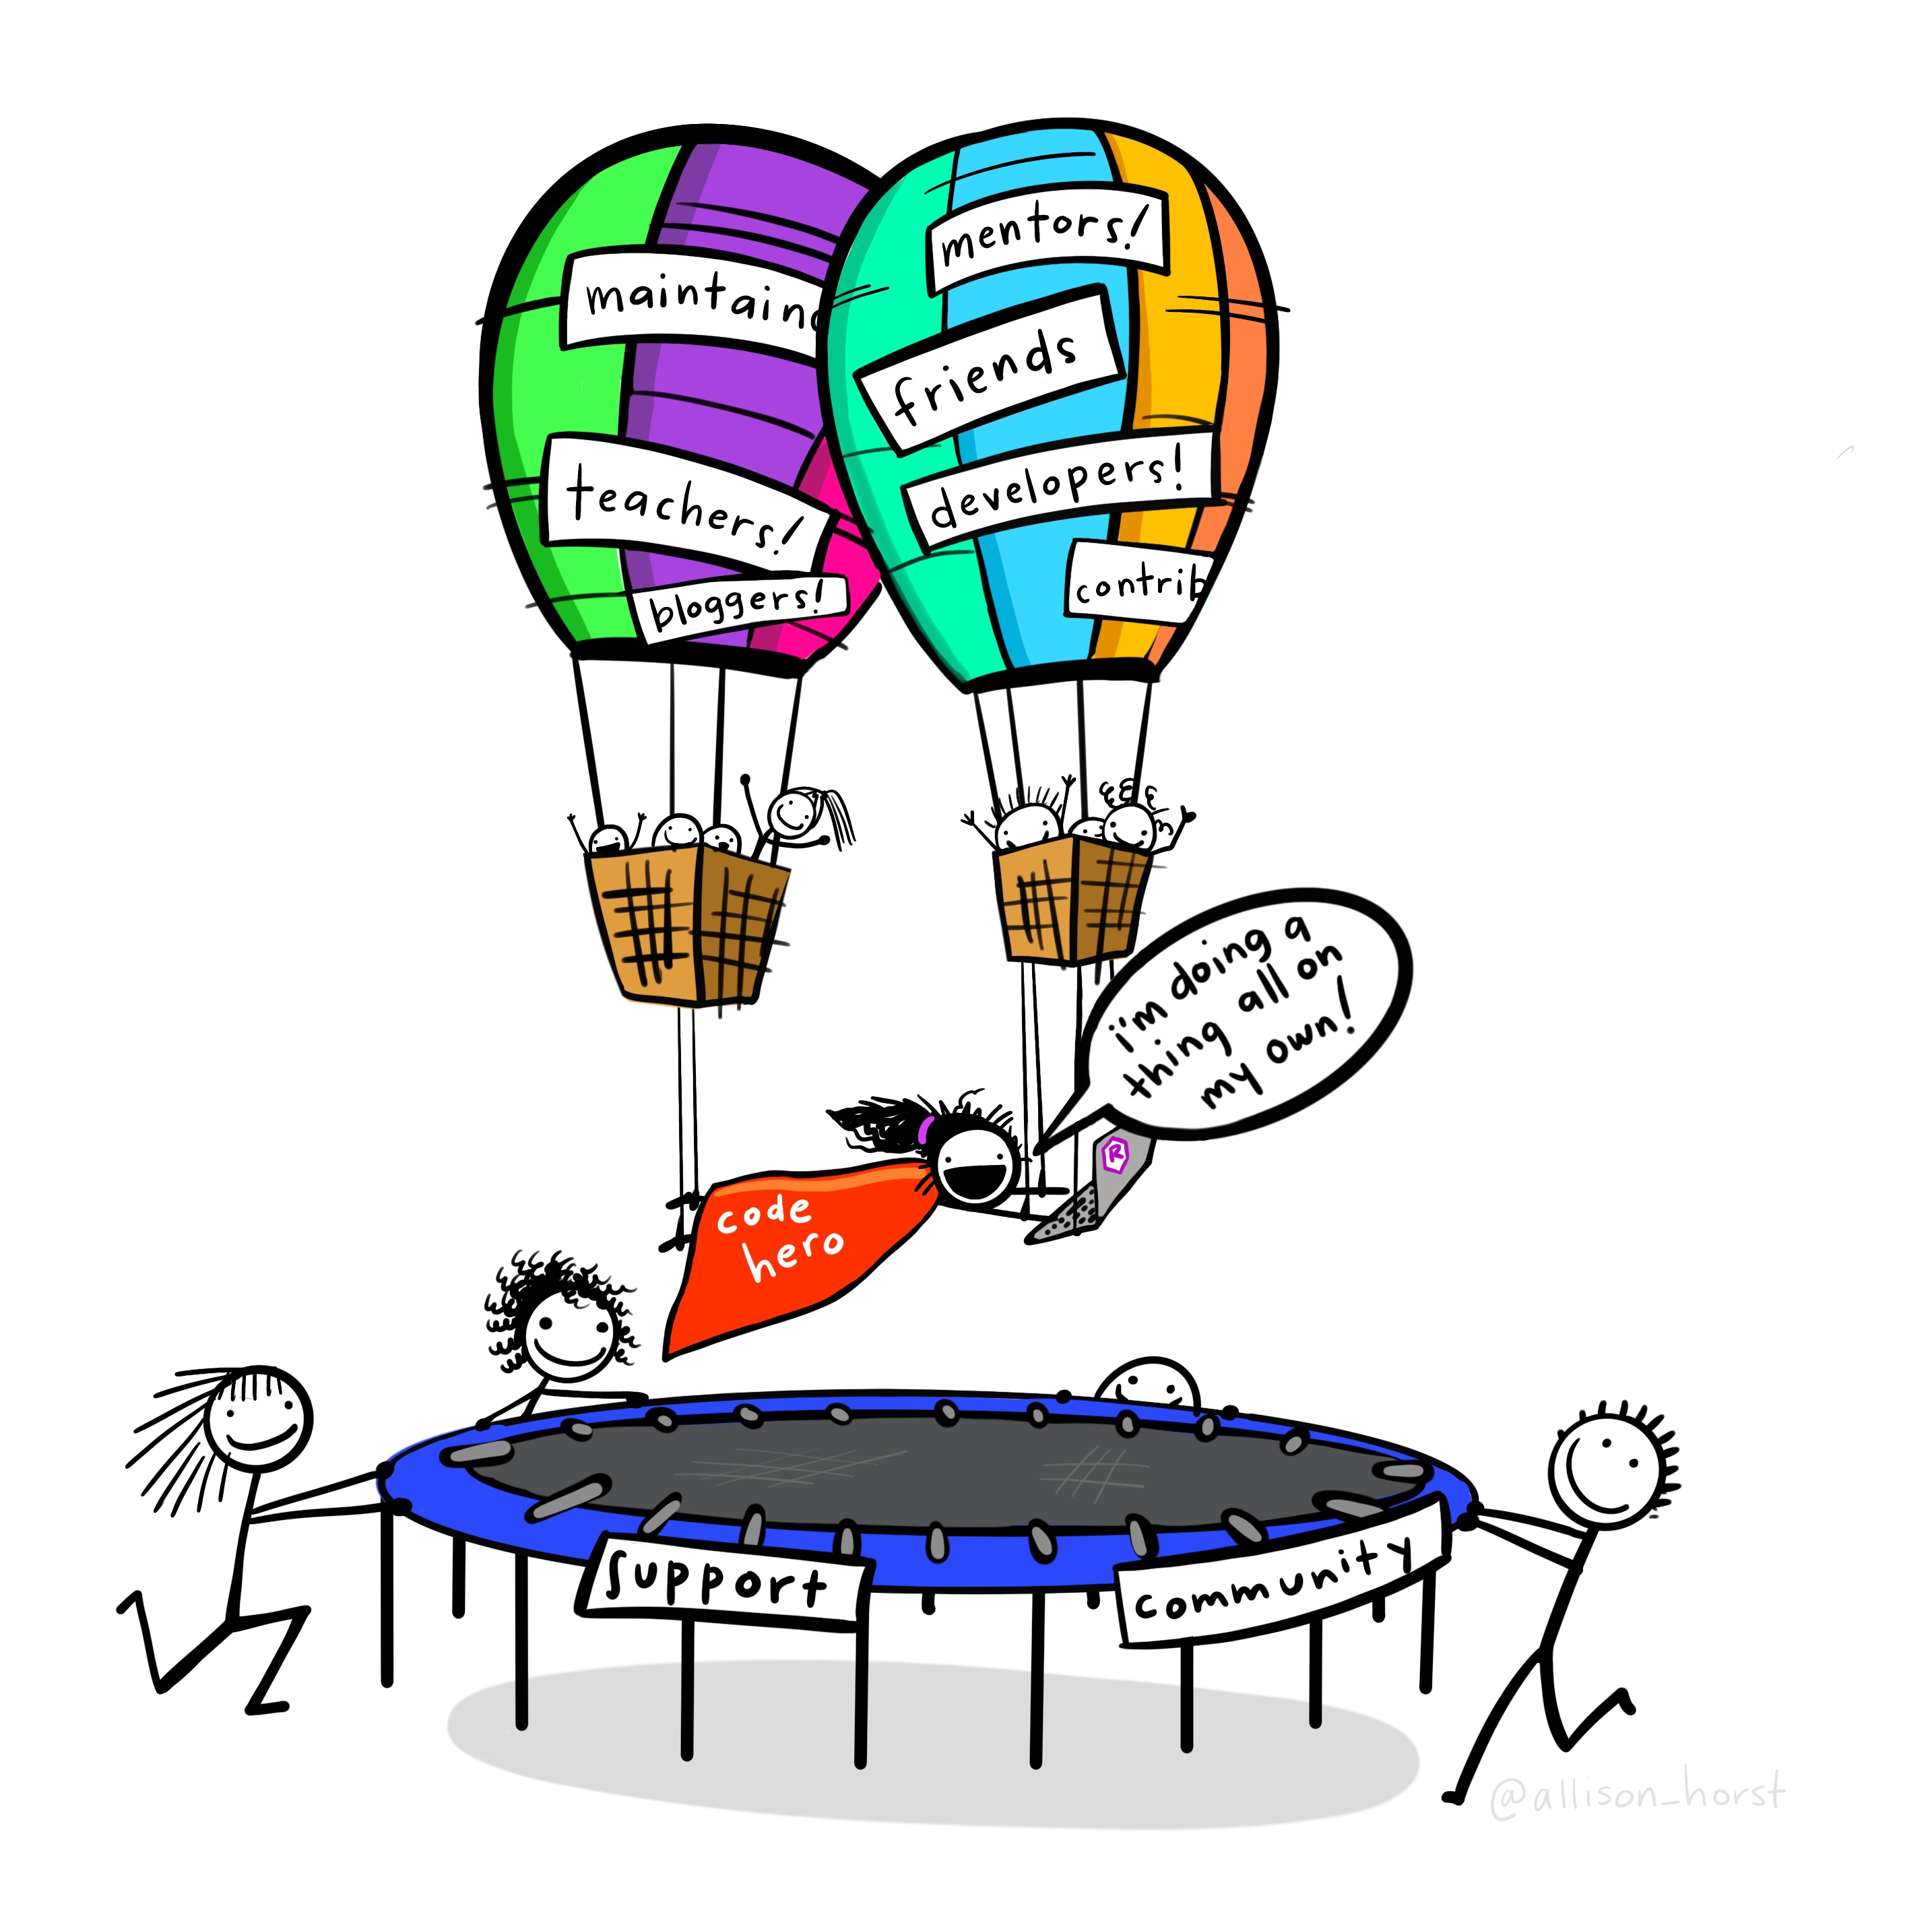
\includegraphics{extfiles/code_hero.jpg}
\caption{Illustrating standing on the shoulders of giants: Artwork by
'@'allison\_horst}
\end{figure}

\section{External R resources that might be
helpful}\label{external-r-resources-that-might-be-helpful}

We provide here a small list of these that might be particularly helpful
for beginners:

\begin{itemize}
\item
  \href{http://r-project.org}{R webpage} - the main R webpage, including
  links to downloading R, manuals, tutorials, dedicated search engines,
  etc.
\item
  \href{https://swirlstats.com/}{Swirl} - if you want to learn R
  interactively from the command line, you might want to try this
  package. Your own R tutor at your fingertips. Try it!
\item
  \href{http://blog.revolutionanalytics.com/2013/08/google-video-r-tutorials.html}{R
  video tutorials} - video how to's in R
\item
  \href{http://www.datamind.org/}{Online tutorial} - a course with
  interactive exercises
\item
  \href{http://faculty.washington.edu/tlumley/Rcourse/}{Online course} -
  notes for a two-day course in R
\item
  \href{http://cran.r-project.org/doc/contrib/refcard.pdf}{Reference
  card} - A very handy list of useful R functions
\item
  \href{http://cran.r-project.org/doc/contrib/Short-refcard.pdf}{Short
  reference card} - A longer reference card with most commonly used R
  functions
\item
  \href{https://www.rstudio.com/resources/cheatsheets/}{Cheat sheets} -
  an incredible useful set of resources from the RStudio team, where
  self contained subject specific sets of functions are provided for
  different common tasks
\end{itemize}

At the landing page of the github repository hosting this tutorial

\url{https://github.com/TiagoAMarques/AnIntro2RTutorial}

there is a longer list of less introductory/general resources on R that
might just have what you were looking for. Disclaimer: said list
corresponds to a random non-exhaustive list of resources I have read and
were useful to me at some point. I make no claims they might be useful
to you :)

\section{Introduction to RStudio}\label{introduction-to-rstudio}

Typically, if I am using this tutorial in a class room, the student will
have been exposed to the PowerPoint
\texttt{Quick\ introduction\ to\ R\ and\ RStudio.pptx}. If you are not
in a class room, you might want to take a look at it. This is also
available at the repository

\url{https://github.com/TiagoAMarques/AnIntro2RTutorial}

right about
\href{https://github.com/TiagoAMarques/AnIntro2RTutorial/blob/0db9070cb440ea591a74744c64c17e3022830f43/Quick\%20introduction\%20to\%20R\%20and\%20R\%20Studio.pptx}{here}.

Nowadays most users (except perhaps die hard command line users) will
use some sort of graphical user interface (GUI) to R. While the basic R
installation comes with a simple GUI, here we adopt the use of RStudio,
which considerably facilitates an introduction to R by providing many
shortcuts and convenient features which we introduce next.

A major advantage of RStudio is that it makes it easy for you to type
your R code into a script window, which you can easily save, and then
send individual lines or blocks of code to the R command line to be
acted upon. This way, you have a record of what you have done, in the
saved script file, and can easily reproduce it any time you like. We
strongly recommend that you save your code script.

Given RStudio has been installed, when you double-click on a R workspace
it should open in RStudio. Note that, if this fails, you might have to
first associate .Rdata files with RStudio. After the presentation on R
and RStudio you just sat through, from within RStudio you should be able
to know where to find:

\begin{itemize}
\tightlist
\item
  the command line (bottom left pane
  \footnote{All the tab positions are the RStudio defaults, but this can be customized by the user later.})
\item
  the code scripts (top left pane)
\item
  the workspace objects (top right pane)
\item
  the loaded packages and how to load them (bottom right pane)
\item
  the created plots (bottom right pane)
\item
  the help files (bottom right pane)
\item
  a file navigator system akin to windows explorer (bottom right pane)
\end{itemize}

Note that you can customize the aspect of RStudio (e.g.~font size and
colors of the smart syntax highlighting scheme) via
``Tools\textbar Global options''.

A very handy feature of RStudio is that you can preview the possible
arguments of functions, as well as their description, directly when you
are inserting the code. Let's try doing that. Type say \texttt{seq()} in
the command line or the script window and then place the cursor between
the parenthesis and press the ``Tab'' key\ldots{} Is this a nice feature
or what?

Now we have met RStudio and we know how it can make our life simpler,
let's move on.

\subsection{Dynamic reports and reproducible
research}\label{dynamic-reports-and-reproducible-research}

One of the most amazing features of the integration of R and RStudio is
how simple it becomes to work with dynamic reports, built on RMarkdown.
This will take you to the next level in data analysis! Actually, this
document was itself created as a dynamic report, using RMarkdown. You
should explore some of the basics of R Markdown, and you can do so here:
\url{https://rmarkdown.rstudio.com/authoring_basics.html}. You can find
additional details here: \url{https://rmarkdown.rstudio.com/}. You can
read an entire free book on the topic here:
\url{https://bookdown.org/yihui/rmarkdown/}.

Experiment yourself to create one. In RStudio, select File -
\textgreater{} New file -\textgreater{} R Markdown\ldots, then just add
a title, something like ``My first dynamic report'' and see what
happens. Explore the content of the file just created and see what
happens when you press the RStudio button \texttt{knit}. Experiment with
the created document to try and change some of the output. Experiment in
creating output as an html, as a pdf, and even as a Word document.

Actually, a good way to learn and get up and running fast in RMarkdown
is by example. Hence, I have prepared a template that you can use to
create without effort a nice dynamic report. Feel free to explore the
material here:

\url{https://github.com/TiagoAMarques/RMarkdownTemplate}

Just download all the files into a folder, \texttt{knit} the file
\texttt{RMarkdownTemplate.Rmd} and off you go.

Imagine the potential when you are analyzing real data, and the data
changes after your report is written!

A recent (well, on the 15th January 2021 it was recent. This wording
might not age well!) note about latest features in RMarkdown is
\href{https://blog.rstudio.com/2020/12/21/rmd-news/}{here}.

\section{A first quick session in
RStudio}\label{a-first-quick-session-in-rstudio}

Here we present a brief introduction to R inside RStudio, using a script
and the command line. In the coming sections we will mostly consider
analysis using dynamic reports via RMarkdown documents (.Rmd), but it is
useful to start with a session where you can see objects being created
in the global environment.

Open RStudio. By default an empty workspace should appear. If you have
an existing workspace, you can open it by selecting
\texttt{File\textbar{}Open\ File}. We recommend that you begin by
creating a script file (\texttt{Ctrl+Shift+N}, RStudio Shortcut) and use
that to save and comment all your code that will be executed during the
tutorial. In this way you will have a record of everything you did.

You know that R is ready to receive a command when you see the R prompt
on the command line (on the bottom left tab by default in RStudio):
\texttt{\textgreater{}}. If you type a line of code that is not
complete, R presents the \texttt{+} character, so that the user knows it
expects the conclusion of the current line.

\textbf{Important note}: while the prompt \texttt{\textgreater{}} and
\texttt{+} might not be shown in this tutorial's code, they are often
present in material online. You should not try to add either
\texttt{\textgreater{}} nor \texttt{+} to the command line: this is
something that R does for you and will complain if you try to do it
yourself! Past experience tells us that more than one person will have
problems because they forgot to delete a \texttt{\textgreater{}} and/or
\texttt{+} from code when they copy paste the code into their own R
sessions. Avoid being that person!

On the top right corner tab, where objects available in the
\texttt{Environment} are listed, given this is a fresh R session, you
currently have no objects.

Here we just create a couple of objects and use them, but below we will
do it again in more detail. Now we just want to create some objects so
that we can then save them and retrieve them again.

\begin{Shaded}
\begin{Highlighting}[]
\CommentTok{\# assign the value 3 to the object hh2}
\NormalTok{hh2}\OtherTok{\textless{}{-}}\DecValTok{3}
\CommentTok{\# assign the value 5 to the object hh3}
\NormalTok{hh3}\OtherTok{\textless{}{-}}\DecValTok{5}
\CommentTok{\# multiply them up}
\NormalTok{hh2}\SpecialCharTok{*}\NormalTok{hh3}
\end{Highlighting}
\end{Shaded}

\begin{verbatim}
## [1] 15
\end{verbatim}

\begin{Shaded}
\begin{Highlighting}[]
\CommentTok{\# add them up}
\NormalTok{hh2}\SpecialCharTok{+}\NormalTok{hh3}
\end{Highlighting}
\end{Shaded}

\begin{verbatim}
## [1] 8
\end{verbatim}

\begin{Shaded}
\begin{Highlighting}[]
\CommentTok{\#note how you can write comments in R by using "\#"}
\CommentTok{\#anything in front of \# is not interpreted by R}
\CommentTok{\#and treated as a comment}
\CommentTok{\#you should have the good habit of extensively commenting}
\CommentTok{\#all your code so that you know what you\textquotesingle{}ve done}
\CommentTok{\#when you return to it even months or years later}
\end{Highlighting}
\end{Shaded}

We can print an object to the screen by simply typing its name and press
enter (despite the fact that currently you can actually see the values
on these objects \texttt{Environment} tab - but that is because they are
simple objects and the workspace is almost empty.).

\begin{Shaded}
\begin{Highlighting}[]
\NormalTok{hh2}
\end{Highlighting}
\end{Shaded}

\begin{verbatim}
## [1] 3
\end{verbatim}

\begin{Shaded}
\begin{Highlighting}[]
\CommentTok{\#same as }
\FunctionTok{print}\NormalTok{(hh2)}
\end{Highlighting}
\end{Shaded}

\begin{verbatim}
## [1] 3
\end{verbatim}

Tip: There is actually a simpler way to execute code from the script
file in RStudio. \texttt{CTRL-Enter} is a keyboard shortcut for ``source
the current line of code in my script file and move the cursor to the
next line''. In general if you like keyboard shortcuts, look in RStudio
under the menu \texttt{Help\ \textbar{}\ Keyboard\ shortcuts} - there
are probably many more than those you will be able to remember!

R is a very powerful calculator! Try some simple maths, say for example
(you need to press enter after each line so that the line is evaluated)

\begin{Shaded}
\begin{Highlighting}[]
\CommentTok{\# R can add!}
\DecValTok{4}\SpecialCharTok{+}\DecValTok{3}
\end{Highlighting}
\end{Shaded}

\begin{verbatim}
## [1] 7
\end{verbatim}

\begin{Shaded}
\begin{Highlighting}[]
\CommentTok{\# and calculate a logarithm (here, of 8)}
\FunctionTok{log}\NormalTok{(}\DecValTok{8}\NormalTok{)}
\end{Highlighting}
\end{Shaded}

\begin{verbatim}
## [1] 2.079442
\end{verbatim}

\begin{Shaded}
\begin{Highlighting}[]
\CommentTok{\#calculates the sin of a number (here of 3.1415)}
\FunctionTok{sin}\NormalTok{(pi)}
\end{Highlighting}
\end{Shaded}

\begin{verbatim}
## [1] 1.224606e-16
\end{verbatim}

\begin{Shaded}
\begin{Highlighting}[]
\CommentTok{\# or make any kind of calculation really}
\DecValTok{1234}\SpecialCharTok{*}\FunctionTok{sqrt}\NormalTok{(}\DecValTok{234}\NormalTok{)}\SpecialCharTok{{-}}\DecValTok{12}\SpecialCharTok{/}\DecValTok{23}\SpecialCharTok{*}\DecValTok{4}\SpecialCharTok{\^{}}\NormalTok{(}\FloatTok{0.12{-}0.4}\NormalTok{)}
\end{Highlighting}
\end{Shaded}

\begin{verbatim}
## [1] 18876.22
\end{verbatim}

R will do much more than that, of course. But it can be hard to get
going. There will be hundreds or thousands of functions to choose from.
The \texttt{print}, \texttt{log} and \texttt{sin} above were just three
examples. If you want to know how to use a function, RStudio provides a
very useful auto-completion code capability. Try to write this on the
command line

\begin{Shaded}
\begin{Highlighting}[]
\FunctionTok{log}\NormalTok{()}
\end{Highlighting}
\end{Shaded}

and then put the cursor inside the function parenthesis and press the
\texttt{Tab} key. RStudio will show you what are the arguments that the
function can take (in this case, it's just the number you want the
logarithm for, \texttt{x}, and \texttt{base}, the base of the respective
logarithm). Remember this when you are using functions and unsure of
what the corresponding arguments are.

It is now time to end our first R session. At this point you need to
decide what to do, as all objects created so far are in the memory, but
this will be wiped out unless we explicitly save it to a file. The
easiest way to do so is by calling the \texttt{save.image} function

\begin{Shaded}
\begin{Highlighting}[]
\FunctionTok{save.image}\NormalTok{(}\AttributeTok{file=}\StringTok{"my1stR.Rdata"}\NormalTok{)}
\end{Highlighting}
\end{Shaded}

Note the unusual extension name \texttt{.Rdata} associated with R
workspaces (an R file is called a workspace). We could now load up this
workspace in a new R session, or typically we will load up that
workspace by starting R by double clicking on the file created. Do this
to see that you retrieve the above created objects. Note that if you
already have an R session open, you can load up any previously saved
workspace via function \texttt{load}.

Finally, just to avoid clutter later, we will delete all the objects
created so far

\begin{Shaded}
\begin{Highlighting}[]
\CommentTok{\#deletes all objects in the dynamic report temporary memory}
\FunctionTok{rm}\NormalTok{(}\AttributeTok{list =} \FunctionTok{ls}\NormalTok{())}
\end{Highlighting}
\end{Shaded}

Note that you have saved your workspace in some directory but you have
not defined the directory explicitly. By default, this is your working
directory. You can check what that directory currently is by using the
following command

\begin{Shaded}
\begin{Highlighting}[]
\FunctionTok{getwd}\NormalTok{()}
\end{Highlighting}
\end{Shaded}

\begin{verbatim}
## [1] "C:/Users/tam2/Dropbox/GithubProjects/AnIntro2RTutorial"
\end{verbatim}

You can always change the directory you are working on by setting it up
explicitly to your desired location, using

\begin{Shaded}
\begin{Highlighting}[]
\CommentTok{\#set the working directory {-} but remember to use your own path!!!}
\FunctionTok{setwd}\NormalTok{(}\StringTok{"C:/Users/tiago/Desktop/mycourse"}\NormalTok{)}
\end{Highlighting}
\end{Shaded}

It is a very good habit to make sure that you are working in the
directory you think you are working. Many errors might occur if R can't
find some object or file because it is looking on the wrong place.

A good trick to make sure you are working in the directory you want is
to open RStudio from the directory you want it to be working on. You can
do that by double clicking a file R studio recognizes as a file it
should open, e.g.~as might happen in particular for files with
extensions .R (a script), a .Rdata (a workspace) or a .Rmd (a dynamic
report in RMarkdown).

If you are already in RStudio, you can also use the \texttt{Files} tab
to see where you are, move to the folder where you want to be working,
and then from the \texttt{Files\textbar{}More} menu (a dented wheel)
select the option \texttt{Set\ as\ working\ directory}.

Now you have used R in RStudio, let's use the power of their integration
to work directly in a dynamic report.

\section{Working through R via a dynamic
report}\label{working-through-r-via-a-dynamic-report}

Create a new dynamic report using a RMarkdown file, as described above.
Comment all you do in the appropriate place. At the end you will have a
record that makes it easy to track everything you did, and a template
you can use in future classes.

Once you created the RMarkdown from scratch, we can start by creating a
new variable.

Note that all the code must go inside code chunks, and you can get them
by doing \texttt{Code\ \textbar{}\ InsertChunk} or the shortcut
\texttt{Ctrl+Alt+I}.

An empty code chunk (in the image with a comment added to it!) looks
like this:


\includegraphics{codechunk.JPG}

We will create a variable called \texttt{myvar1} which we will assign
the value of 4. This is typically done using the assign operator
\texttt{\textless{}-}.

\begin{Shaded}
\begin{Highlighting}[]
\NormalTok{myvar1}\OtherTok{\textless{}{-}}\DecValTok{4}
\end{Highlighting}
\end{Shaded}

There are typically multiple ways to do the same thing in R, and this is
sometimes referred to as a disadvantage. For simplicity, we deliberately
avoid presenting the several alternatives for each action, and
concentrate on the ones we prefer. This is not the same as saying these
are the best, and if you continue to work with R you will likely get
used to doing things your way - for now we do it our way!

An object should have been created in your workspace. You can list all
objects in a given workspace using

\begin{Shaded}
\begin{Highlighting}[]
\FunctionTok{ls}\NormalTok{()}
\end{Highlighting}
\end{Shaded}

\begin{verbatim}
## [1] "myvar1"
\end{verbatim}

You can also remove any object by using the\texttt{rm} function, so here
we remove \texttt{myvar1}.

\begin{Shaded}
\begin{Highlighting}[]
\FunctionTok{rm}\NormalTok{(myvar1)}
\end{Highlighting}
\end{Shaded}

and hence our workspace is empty again.

\textbf{Task 0}: Create some objects and assign numbers to them. Then
try to make some basic calculations with the objects you just created.
Finally, clean up the workspace again.

Note a key difference between the functions \texttt{ls} and \texttt{rm}.
While the first function does not need any arguments, the second
requires at least one argument (but can take several). This can be
easily seen by checking their help files and noting that \texttt{rm}
needs at least 1 explicit argument while \texttt{ls} can work with
defaults

\begin{Shaded}
\begin{Highlighting}[]
\NormalTok{?rm}
\end{Highlighting}
\end{Shaded}

This is a convenient way to obtain more information about a given
function. If one does not know what the name of the function might be,
one can search for functions containing a given string. The following
command lists all the functions with the string \texttt{mean} in them.

\begin{Shaded}
\begin{Highlighting}[]
\FunctionTok{apropos}\NormalTok{(}\StringTok{"mean"}\NormalTok{)}
\end{Highlighting}
\end{Shaded}

\begin{verbatim}
##  [1] ".colMeans"     ".rowMeans"     "colMeans"      "kmeans"       
##  [5] "mean"          "mean.Date"     "mean.default"  "mean.difftime"
##  [9] "mean.POSIXct"  "mean.POSIXlt"  "rowMeans"      "weighted.mean"
\end{verbatim}

Not surprisingly, most if not all of these functions will be used for
some kind of calculation involving a mean. You can look into any one of
them using the \texttt{?} as above. We have assigned a number to a
variable , but we can actually more generally have vectors (strictly,
\texttt{myvar1} was a numeric vector of length 1) containing a large
number of values ``inside'' them.

The following code assigns some numbers to 5 different vectors.

\begin{Shaded}
\begin{Highlighting}[]
\NormalTok{x2}\OtherTok{\textless{}{-}}\FunctionTok{c}\NormalTok{(}\DecValTok{1}\NormalTok{,}\DecValTok{2}\NormalTok{,}\FloatTok{0.12}\NormalTok{,}\DecValTok{4}\NormalTok{,}\SpecialCharTok{{-}}\DecValTok{22}\NormalTok{)}
\NormalTok{x3}\OtherTok{\textless{}{-}}\FunctionTok{seq}\NormalTok{(}\DecValTok{1}\NormalTok{,}\DecValTok{8}\NormalTok{,}\AttributeTok{by=}\DecValTok{2}\NormalTok{)}
\CommentTok{\# : useful shortcut for sequences with the by argument = 1}
\NormalTok{x1}\OtherTok{\textless{}{-}}\DecValTok{1}\SpecialCharTok{:}\DecValTok{5}
\NormalTok{z1}\OtherTok{\textless{}{-}}\DecValTok{10}\SpecialCharTok{:}\DecValTok{8}
\NormalTok{z2}\OtherTok{\textless{}{-}}\SpecialCharTok{{-}}\DecValTok{10}\SpecialCharTok{:}\DecValTok{10}
\end{Highlighting}
\end{Shaded}

Take a peak at the objects just created:

\begin{Shaded}
\begin{Highlighting}[]
\NormalTok{x1}
\end{Highlighting}
\end{Shaded}

\begin{verbatim}
## [1] 1 2 3 4 5
\end{verbatim}

\begin{Shaded}
\begin{Highlighting}[]
\NormalTok{x2}
\end{Highlighting}
\end{Shaded}

\begin{verbatim}
## [1]   1.00   2.00   0.12   4.00 -22.00
\end{verbatim}

\begin{Shaded}
\begin{Highlighting}[]
\NormalTok{x3}
\end{Highlighting}
\end{Shaded}

\begin{verbatim}
## [1] 1 3 5 7
\end{verbatim}

\begin{Shaded}
\begin{Highlighting}[]
\NormalTok{z1}
\end{Highlighting}
\end{Shaded}

\begin{verbatim}
## [1] 10  9  8
\end{verbatim}

\begin{Shaded}
\begin{Highlighting}[]
\NormalTok{z2}
\end{Highlighting}
\end{Shaded}

\begin{verbatim}
##  [1] -10  -9  -8  -7  -6  -5  -4  -3  -2  -1   0   1   2   3   4   5   6   7   8
## [20]   9  10
\end{verbatim}

The function \texttt{seq} is very useful for setting sequences of
numbers. The optional arguments \texttt{length.out} and
\texttt{along.with} provide extra flexibility. Look at \texttt{?seq} to
find out what the function does and the consequences of using these
different arguments.

We can use the usual mathematical operators over vectors. A few examples
follow:

\begin{Shaded}
\begin{Highlighting}[]
\NormalTok{x1}\SpecialCharTok{+}\NormalTok{x2}
\end{Highlighting}
\end{Shaded}

\begin{verbatim}
## [1]   2.00   4.00   3.12   8.00 -17.00
\end{verbatim}

\begin{Shaded}
\begin{Highlighting}[]
\NormalTok{x4}\OtherTok{\textless{}{-}}\NormalTok{x1}\SpecialCharTok{+}\NormalTok{x2}
\NormalTok{x5}\OtherTok{\textless{}{-}}\NormalTok{x1}\SpecialCharTok{{-}}\NormalTok{x2}
\NormalTok{x6}\OtherTok{\textless{}{-}}\NormalTok{x1}\SpecialCharTok{*}\NormalTok{x2}
\NormalTok{x7}\OtherTok{\textless{}{-}}\NormalTok{x1}\SpecialCharTok{/}\NormalTok{x2}
\end{Highlighting}
\end{Shaded}

Note by default you do not see results, you need to print them to the
report to see them. As an example

\begin{Shaded}
\begin{Highlighting}[]
\FunctionTok{print}\NormalTok{(x4)}
\end{Highlighting}
\end{Shaded}

\begin{verbatim}
## [1]   2.00   4.00   3.12   8.00 -17.00
\end{verbatim}

it is actually simpler than using print, because if you just use the
name of the object on the console it gets printed by default

\begin{Shaded}
\begin{Highlighting}[]
\NormalTok{x4}
\end{Highlighting}
\end{Shaded}

\begin{verbatim}
## [1]   2.00   4.00   3.12   8.00 -17.00
\end{verbatim}

\begin{Shaded}
\begin{Highlighting}[]
\NormalTok{x5}
\end{Highlighting}
\end{Shaded}

\begin{verbatim}
## [1]  0.00  0.00  2.88  0.00 27.00
\end{verbatim}

\begin{Shaded}
\begin{Highlighting}[]
\NormalTok{x6}
\end{Highlighting}
\end{Shaded}

\begin{verbatim}
## [1]    1.00    4.00    0.36   16.00 -110.00
\end{verbatim}

\begin{Shaded}
\begin{Highlighting}[]
\NormalTok{x7}
\end{Highlighting}
\end{Shaded}

\begin{verbatim}
## [1]  1.0000000  1.0000000 25.0000000  1.0000000 -0.2272727
\end{verbatim}

Note that if the vectors are of the same length, R performs the
operation element-wise. Another useful (but possibly dangerous) feature
is that R recycles vectors if they are not the same length

\begin{Shaded}
\begin{Highlighting}[]
\NormalTok{x8}\OtherTok{\textless{}{-}}\FunctionTok{c}\NormalTok{(}\DecValTok{1}\NormalTok{,}\DecValTok{2}\NormalTok{,}\DecValTok{3}\NormalTok{,}\DecValTok{4}\NormalTok{)}
\NormalTok{x8}\SpecialCharTok{+}\DecValTok{2}
\end{Highlighting}
\end{Shaded}

\begin{verbatim}
## [1] 3 4 5 6
\end{verbatim}

However, if one of the vectors is smaller, unexpected behavior can
happen, because R recycles elements regardless (so be careful, a warning
is typically produced)

\begin{Shaded}
\begin{Highlighting}[]
\NormalTok{x9}\OtherTok{\textless{}{-}}\FunctionTok{c}\NormalTok{(}\DecValTok{3}\NormalTok{,}\DecValTok{4}\NormalTok{,}\DecValTok{5}\NormalTok{)}
\NormalTok{x10}\OtherTok{\textless{}{-}}\FunctionTok{c}\NormalTok{(}\FloatTok{0.7}\NormalTok{,}\FloatTok{0.9}\NormalTok{,}\FloatTok{1.3}\NormalTok{)}
\NormalTok{x9}\SpecialCharTok{+}\NormalTok{x10}
\end{Highlighting}
\end{Shaded}

\begin{verbatim}
## [1] 3.7 4.9 6.3
\end{verbatim}

\begin{Shaded}
\begin{Highlighting}[]
\NormalTok{x8}\SpecialCharTok{+}\NormalTok{x9}
\end{Highlighting}
\end{Shaded}

\begin{verbatim}
## Warning in x8 + x9: longer object length is not a multiple of shorter object
## length
\end{verbatim}

\begin{verbatim}
## [1] 4 6 8 7
\end{verbatim}

As expected, a warning message was produced when \texttt{x8} and
\texttt{x9} were added. Usually \emph{these messages are important and
should be read}! Quite often the answer to your current question lies in
the previous error or warning message.

Another useful function is \texttt{rep}, which allows one to create
repetitions of patterns. As examples, see the difference between the
next two lines of code

\begin{Shaded}
\begin{Highlighting}[]
\FunctionTok{rep}\NormalTok{(}\FunctionTok{c}\NormalTok{(}\DecValTok{1}\NormalTok{,}\DecValTok{2}\NormalTok{,}\DecValTok{3}\NormalTok{,}\DecValTok{4}\NormalTok{),}\AttributeTok{times=}\DecValTok{3}\NormalTok{)}
\end{Highlighting}
\end{Shaded}

\begin{verbatim}
##  [1] 1 2 3 4 1 2 3 4 1 2 3 4
\end{verbatim}

\begin{Shaded}
\begin{Highlighting}[]
\FunctionTok{rep}\NormalTok{(}\FunctionTok{c}\NormalTok{(}\DecValTok{1}\NormalTok{,}\DecValTok{2}\NormalTok{,}\DecValTok{3}\NormalTok{,}\DecValTok{4}\NormalTok{),}\AttributeTok{each=}\DecValTok{3}\NormalTok{)}
\end{Highlighting}
\end{Shaded}

\begin{verbatim}
##  [1] 1 1 1 2 2 2 3 3 3 4 4 4
\end{verbatim}

We have just started R, created and removed some objects, and used
simple functions like \texttt{ls}, \texttt{seq} or \texttt{save}. R is
an object oriented language, and functions and vectors are just examples
of types of objects available in R. In the next section we go through
the most commonly used classes of objects in R.

\subsection{Types and classes of
objects}\label{types-and-classes-of-objects}

Objects can have classes, which allow functions to interact with them.
Objects can be of several classes. We already used the class
\texttt{numeric}, which is used for general numbers, but there are also
additional very commonly used classes:

\begin{itemize}
\tightlist
\item
  \texttt{integer}, for integer numbers
\item
  \texttt{character}, just for character strings
\item
  \texttt{factor}, used to represent levels of a categorical variable
\item
  \texttt{logical}, the values TRUE and FALSE
\end{itemize}

While many others exist, these are the more commonly used. Another type
of object which we have already used are functions.

\begin{Shaded}
\begin{Highlighting}[]
\FunctionTok{class}\NormalTok{(mean)}
\end{Highlighting}
\end{Shaded}

\begin{verbatim}
## [1] "function"
\end{verbatim}

While there are thousands of available functions inside R, later we will
learn how to create our own functions.

Outputs of some analyses have special classes, as an example, the output
of a call of function \texttt{lm} is an object of class \texttt{lm},
i.e., a linear model. Many packages introduce special classes for
objects, so that functions know how to behave when those objects are
used as arguments. Typically, functions behave differently according to
the class of the objects that are used as arguments to them. As an
example, note how \texttt{summary} treats differently an object of class
\texttt{factor} or one of class \texttt{numeric}, producing a table of
counts per level for a factor but a 6 number summary for numeric values.

\begin{Shaded}
\begin{Highlighting}[]
\NormalTok{obj1}\OtherTok{\textless{}{-}}\FunctionTok{factor}\NormalTok{(}\FunctionTok{c}\NormalTok{(}\FunctionTok{rep}\NormalTok{(}\StringTok{"a"}\NormalTok{,}\DecValTok{12}\NormalTok{),}\FunctionTok{rep}\NormalTok{(}\StringTok{"b"}\NormalTok{,}\DecValTok{4}\NormalTok{),}\FunctionTok{rep}\NormalTok{(}\StringTok{"c"}\NormalTok{,}\DecValTok{2}\NormalTok{)))}
\FunctionTok{summary}\NormalTok{(obj1)}
\end{Highlighting}
\end{Shaded}

\begin{verbatim}
##  a  b  c 
## 12  4  2
\end{verbatim}

\begin{Shaded}
\begin{Highlighting}[]
\NormalTok{obj2}\OtherTok{\textless{}{-}}\FunctionTok{c}\NormalTok{(}\DecValTok{2}\NormalTok{,}\DecValTok{5}\NormalTok{,}\SpecialCharTok{{-}}\FloatTok{0.2}\NormalTok{,}\DecValTok{89}\NormalTok{,}\DecValTok{12}\NormalTok{,}\SpecialCharTok{{-}}\DecValTok{3}\NormalTok{,}\SpecialCharTok{{-}}\FloatTok{5.4}\NormalTok{)}
\FunctionTok{summary}\NormalTok{(obj2)}
\end{Highlighting}
\end{Shaded}

\begin{verbatim}
##    Min. 1st Qu.  Median    Mean 3rd Qu.    Max. 
##    -5.4    -1.6     2.0    14.2     8.5    89.0
\end{verbatim}

We can check the class of an object using function \texttt{class}, as in
the following examples

\begin{Shaded}
\begin{Highlighting}[]
\FunctionTok{class}\NormalTok{(obj1)}
\end{Highlighting}
\end{Shaded}

\begin{verbatim}
## [1] "factor"
\end{verbatim}

\begin{Shaded}
\begin{Highlighting}[]
\FunctionTok{class}\NormalTok{(obj2)}
\end{Highlighting}
\end{Shaded}

\begin{verbatim}
## [1] "numeric"
\end{verbatim}

\begin{Shaded}
\begin{Highlighting}[]
\FunctionTok{class}\NormalTok{(}\ConstantTok{TRUE}\NormalTok{)}
\end{Highlighting}
\end{Shaded}

\begin{verbatim}
## [1] "logical"
\end{verbatim}

It is sometimes useful to coerce, i.e.~force, objects into different
classes, but care should be used when doing so. Some examples are
presented below. Can you describe in your own words what R did below?

\begin{Shaded}
\begin{Highlighting}[]
\FunctionTok{as.integer}\NormalTok{(}\FunctionTok{c}\NormalTok{(}\DecValTok{3}\NormalTok{,}\SpecialCharTok{{-}}\FloatTok{0.3}\NormalTok{,}\FloatTok{0.4}\NormalTok{,}\FloatTok{0.6}\NormalTok{,}\FloatTok{0.9}\NormalTok{,}\FloatTok{13.2}\NormalTok{,}\DecValTok{12}\NormalTok{))}
\end{Highlighting}
\end{Shaded}

\begin{verbatim}
## [1]  3  0  0  0  0 13 12
\end{verbatim}

\begin{Shaded}
\begin{Highlighting}[]
\FunctionTok{as.numeric}\NormalTok{(}\FunctionTok{c}\NormalTok{(}\ConstantTok{TRUE}\NormalTok{,}\ConstantTok{FALSE}\NormalTok{,}\ConstantTok{TRUE}\NormalTok{))}
\end{Highlighting}
\end{Shaded}

\begin{verbatim}
## [1] 1 0 1
\end{verbatim}

\begin{Shaded}
\begin{Highlighting}[]
\FunctionTok{as.numeric}\NormalTok{(obj1)}
\end{Highlighting}
\end{Shaded}

\begin{verbatim}
##  [1] 1 1 1 1 1 1 1 1 1 1 1 1 2 2 2 2 3 3
\end{verbatim}

A common way to organize multiple vectors together is in the form of a
matrix. Here we create such an object

\begin{Shaded}
\begin{Highlighting}[]
\NormalTok{mat1}\OtherTok{\textless{}{-}}\FunctionTok{matrix}\NormalTok{(}\DecValTok{1}\SpecialCharTok{:}\DecValTok{12}\NormalTok{,}\AttributeTok{nrow=}\DecValTok{3}\NormalTok{,}\AttributeTok{ncol=}\DecValTok{4}\NormalTok{)}
\NormalTok{mat1}
\end{Highlighting}
\end{Shaded}

\begin{verbatim}
##      [,1] [,2] [,3] [,4]
## [1,]    1    4    7   10
## [2,]    2    5    8   11
## [3,]    3    6    9   12
\end{verbatim}

Note that by default R fills the first column (with 1,2,3) then the
second column (4,5,6) etc. If you want it to fill the first row, then
the second, you can use the optional argument \texttt{byrow=TRUE}, like
this:

\begin{Shaded}
\begin{Highlighting}[]
\FunctionTok{matrix}\NormalTok{(}\DecValTok{1}\SpecialCharTok{:}\DecValTok{12}\NormalTok{,}\AttributeTok{nrow=}\DecValTok{3}\NormalTok{,}\AttributeTok{ncol=}\DecValTok{4}\NormalTok{,}\AttributeTok{byrow=}\ConstantTok{TRUE}\NormalTok{)}
\end{Highlighting}
\end{Shaded}

\begin{verbatim}
##      [,1] [,2] [,3] [,4]
## [1,]    1    2    3    4
## [2,]    5    6    7    8
## [3,]    9   10   11   12
\end{verbatim}

R also allows data structures with more than 2 dimensions -- we don't
cover those here, but look up the help on ``array'\,' if you're
interested. A matrix is just a two dimensional array.

Arrays are useful objects, but can be complex to visualize due to their
potential high dimensionality. Another common type of object is a
\texttt{data.frame}. This is essentially a matrix but for which each
column can be of a different type. These are what we would typically
associate with an excel spreadsheet or a table in a database. Typically
columns correspond to variables observed in a number of subjects, each
subject recorded in its own row. A simple example with 3 variables and 5
subjects follows:

\begin{Shaded}
\begin{Highlighting}[]
\NormalTok{mysex}\OtherTok{\textless{}{-}}\FunctionTok{c}\NormalTok{(}\StringTok{"male"}\NormalTok{,}\StringTok{"female"}\NormalTok{,}\StringTok{"female"}\NormalTok{,}\StringTok{"male"}\NormalTok{,}\StringTok{"male"}\NormalTok{)}
\NormalTok{myage}\OtherTok{\textless{}{-}}\FunctionTok{c}\NormalTok{(}\DecValTok{34}\NormalTok{,}\DecValTok{23}\NormalTok{,}\DecValTok{56}\NormalTok{,}\DecValTok{45}\NormalTok{,}\DecValTok{12}\NormalTok{)}
\NormalTok{myhei}\OtherTok{\textless{}{-}}\FunctionTok{c}\NormalTok{(}\DecValTok{185}\NormalTok{,}\DecValTok{178}\NormalTok{,}\DecValTok{167}\NormalTok{,}\DecValTok{165}\NormalTok{,}\DecValTok{148}\NormalTok{)}
\NormalTok{df1}\OtherTok{\textless{}{-}}\FunctionTok{data.frame}\NormalTok{(}\AttributeTok{ID=}\DecValTok{1}\SpecialCharTok{:}\DecValTok{5}\NormalTok{,}\AttributeTok{sex=}\NormalTok{mysex,}\AttributeTok{age=}\NormalTok{myage,}\AttributeTok{height=}\NormalTok{myhei)}
\NormalTok{df1}
\end{Highlighting}
\end{Shaded}

\begin{verbatim}
##   ID    sex age height
## 1  1   male  34    185
## 2  2 female  23    178
## 3  3 female  56    167
## 4  4   male  45    165
## 5  5   male  12    148
\end{verbatim}

Typically, \texttt{data.frames} are used to store the data we
subsequently analyse. Usually the data are not manually imputed as
above, but read into R from other software, using R functions addressed
in a later section.

A data frame is just a special type of \texttt{list}. A \texttt{list}
can contain objects of different types and dimensions. An example is
here

\begin{Shaded}
\begin{Highlighting}[]
\NormalTok{list1}\OtherTok{\textless{}{-}}\FunctionTok{list}\NormalTok{(}\AttributeTok{Note=}\StringTok{"whatever I want here"}\NormalTok{,}\AttributeTok{X2=}\DecValTok{4}\NormalTok{,}\AttributeTok{age=}\DecValTok{1}\SpecialCharTok{:}\DecValTok{4}\NormalTok{)}
\NormalTok{list1}
\end{Highlighting}
\end{Shaded}

\begin{verbatim}
## $Note
## [1] "whatever I want here"
## 
## $X2
## [1] 4
## 
## $age
## [1] 1 2 3 4
\end{verbatim}

Lists are typically used to store outputs of computations which require
different kinds of objects to be recorded. Note the use of \texttt{\$}
to access the sub components of a list or a data.frame.

\begin{Shaded}
\begin{Highlighting}[]
\NormalTok{list1}\SpecialCharTok{$}\NormalTok{X2}\SpecialCharTok{+}\DecValTok{10}
\end{Highlighting}
\end{Shaded}

\begin{verbatim}
## [1] 14
\end{verbatim}

Alternatively, one might use index to retrieve elements of a list

\begin{Shaded}
\begin{Highlighting}[]
\NormalTok{list1[[}\DecValTok{3}\NormalTok{]]}\SpecialCharTok{+}\DecValTok{5}
\end{Highlighting}
\end{Shaded}

\begin{verbatim}
## [1] 6 7 8 9
\end{verbatim}

In the next section we will learn more about using indexes to access
subsets of data.

\section{Subsetting data}\label{subsetting-data}

One useful feature of R relates to how we can index subsets of data. The
indexing information is included within square
brackets:\texttt{{[}\ {]}}. As an example, we can select the 3rd element
of a vector

\begin{Shaded}
\begin{Highlighting}[]
\NormalTok{x}\OtherTok{\textless{}{-}}\FunctionTok{c}\NormalTok{(}\DecValTok{1}\NormalTok{,}\FloatTok{3.5}\NormalTok{,}\DecValTok{7}\NormalTok{,}\DecValTok{8}\NormalTok{,}\SpecialCharTok{{-}}\DecValTok{7}\NormalTok{,}\FloatTok{0.43}\NormalTok{,}\SpecialCharTok{{-}}\DecValTok{1}\NormalTok{)}
\NormalTok{x[}\DecValTok{3}\NormalTok{]}
\end{Highlighting}
\end{Shaded}

\begin{verbatim}
## [1] 7
\end{verbatim}

but we can also select all except the second and third elements of the
same vector

\begin{Shaded}
\begin{Highlighting}[]
\NormalTok{x[}\SpecialCharTok{{-}}\FunctionTok{c}\NormalTok{(}\DecValTok{2}\NormalTok{,}\DecValTok{3}\NormalTok{)]}
\end{Highlighting}
\end{Shaded}

\begin{verbatim}
## [1]  1.00  8.00 -7.00  0.43 -1.00
\end{verbatim}

We can also select only the objects which follow a given condition, say
only those that are positive

\begin{Shaded}
\begin{Highlighting}[]
\NormalTok{x[x}\SpecialCharTok{\textgreater{}}\DecValTok{0}\NormalTok{]}
\end{Highlighting}
\end{Shaded}

\begin{verbatim}
## [1] 1.00 3.50 7.00 8.00 0.43
\end{verbatim}

\noindent or those between (-1,1)

\begin{Shaded}
\begin{Highlighting}[]
\NormalTok{x[(x}\SpecialCharTok{\textgreater{}{-}}\DecValTok{1}\NormalTok{) }\SpecialCharTok{\&}\NormalTok{ (x}\SpecialCharTok{\textless{}}\DecValTok{1}\NormalTok{)]}
\end{Highlighting}
\end{Shaded}

\begin{verbatim}
## [1] 0.43
\end{verbatim}

Note the subtle difference between the previous and next statements

\begin{Shaded}
\begin{Highlighting}[]
\NormalTok{x[(x}\SpecialCharTok{\textgreater{}={-}}\DecValTok{1}\NormalTok{) }\SpecialCharTok{\&}\NormalTok{ (x}\SpecialCharTok{\textless{}=}\DecValTok{1}\NormalTok{)]}
\end{Highlighting}
\end{Shaded}

\begin{verbatim}
## [1]  1.00  0.43 -1.00
\end{verbatim}

\noindent which reminds us we should be careful when setting these
logical conditions, especially when working with integer boundaries
which might be on the limits of those conditions. Note indexing can be
done using additional information. As an example, we select here the
elements in \texttt{x} such that the corresponding elements in
\texttt{y} are positive:

\begin{Shaded}
\begin{Highlighting}[]
\CommentTok{\#rnorm(k) produces k Gaussian random deviates}
\NormalTok{x}\OtherTok{\textless{}{-}}\FunctionTok{rnorm}\NormalTok{(}\DecValTok{10}\NormalTok{)}
\NormalTok{y}\OtherTok{\textless{}{-}}\FunctionTok{rnorm}\NormalTok{(}\DecValTok{10}\NormalTok{)}
\NormalTok{x2}\OtherTok{\textless{}{-}}\NormalTok{x[y}\SpecialCharTok{\textgreater{}}\DecValTok{0}\NormalTok{]}
\end{Highlighting}
\end{Shaded}

When working on a matrix the indexing is done by row and column,
therefore for selecting the value that is in the third row and second
column of a matrix we use

\begin{Shaded}
\begin{Highlighting}[]
\NormalTok{mat1[}\DecValTok{3}\NormalTok{,}\DecValTok{2}\NormalTok{]}
\end{Highlighting}
\end{Shaded}

\begin{verbatim}
## [1] 6
\end{verbatim}

\noindent but we can also select all the elements in the second row

\begin{Shaded}
\begin{Highlighting}[]
\NormalTok{mat1[}\DecValTok{2}\NormalTok{,]}
\end{Highlighting}
\end{Shaded}

\begin{verbatim}
## [1]  2  5  8 11
\end{verbatim}

or the fourth column

\begin{Shaded}
\begin{Highlighting}[]
\NormalTok{mat1[,}\DecValTok{4}\NormalTok{]}
\end{Highlighting}
\end{Shaded}

\begin{verbatim}
## [1] 10 11 12
\end{verbatim}

We are often interested in subsetting a dataset by some characteristic
of one (or several) of its columns. Here we illustrate with the dataset
\texttt{iris} (check \texttt{?iris} for data details)

\begin{Shaded}
\begin{Highlighting}[]
\FunctionTok{head}\NormalTok{(iris)}
\end{Highlighting}
\end{Shaded}

\begin{verbatim}
##   Sepal.Length Sepal.Width Petal.Length Petal.Width Species
## 1          5.1         3.5          1.4         0.2  setosa
## 2          4.9         3.0          1.4         0.2  setosa
## 3          4.7         3.2          1.3         0.2  setosa
## 4          4.6         3.1          1.5         0.2  setosa
## 5          5.0         3.6          1.4         0.2  setosa
## 6          5.4         3.9          1.7         0.4  setosa
\end{verbatim}

\begin{Shaded}
\begin{Highlighting}[]
\FunctionTok{str}\NormalTok{(iris)}
\end{Highlighting}
\end{Shaded}

\begin{verbatim}
## 'data.frame':    150 obs. of  5 variables:
##  $ Sepal.Length: num  5.1 4.9 4.7 4.6 5 5.4 4.6 5 4.4 4.9 ...
##  $ Sepal.Width : num  3.5 3 3.2 3.1 3.6 3.9 3.4 3.4 2.9 3.1 ...
##  $ Petal.Length: num  1.4 1.4 1.3 1.5 1.4 1.7 1.4 1.5 1.4 1.5 ...
##  $ Petal.Width : num  0.2 0.2 0.2 0.2 0.2 0.4 0.3 0.2 0.2 0.1 ...
##  $ Species     : Factor w/ 3 levels "setosa","versicolor",..: 1 1 1 1 1 1 1 1 1 1 ...
\end{verbatim}

that contains information about 3 species: setosa, versicolor and
virginica. Imagine that we want to do something just with those from
species virginica. Then we can create an object holding just that
information as

\begin{Shaded}
\begin{Highlighting}[]
\NormalTok{iris}\FloatTok{.3} \OtherTok{\textless{}{-}}\NormalTok{ iris[iris}\SpecialCharTok{$}\NormalTok{Species}\SpecialCharTok{==}\StringTok{"virginica"}\NormalTok{,]}
\FunctionTok{summary}\NormalTok{(iris}\FloatTok{.3}\NormalTok{)}
\end{Highlighting}
\end{Shaded}

\begin{verbatim}
##   Sepal.Length    Sepal.Width     Petal.Length    Petal.Width   
##  Min.   :4.900   Min.   :2.200   Min.   :4.500   Min.   :1.400  
##  1st Qu.:6.225   1st Qu.:2.800   1st Qu.:5.100   1st Qu.:1.800  
##  Median :6.500   Median :3.000   Median :5.550   Median :2.000  
##  Mean   :6.588   Mean   :2.974   Mean   :5.552   Mean   :2.026  
##  3rd Qu.:6.900   3rd Qu.:3.175   3rd Qu.:5.875   3rd Qu.:2.300  
##  Max.   :7.900   Max.   :3.800   Max.   :6.900   Max.   :2.500  
##        Species  
##  setosa    : 0  
##  versicolor: 0  
##  virginica :50  
##                 
##                 
## 
\end{verbatim}

\section{Mathematical functions}\label{mathematical-functions}

Within R there are a number of mathematical operators but also
mathematical and statistical functions. As any other functions, many of
these have required parameters and optional parameters. It would take a
very long time to describe even the most basic functions. Therefore, we
prefer to let you try hands on explore a number of these.

\textbf{Task 1}: Take your time to explore the functions below:
\texttt{sum(x)}, \texttt{sqrt(x)}, \texttt{log(x)}, \texttt{log(x,n)},
\texttt{exp(x)}, \texttt{choose(n,x)}, \texttt{factorial(x)},
\texttt{floor(x)}, \texttt{ceiling(x)}, \texttt{round(x,digits)},
\texttt{abs(x)}, \texttt{cos(x)}, \texttt{sin(x)}, \texttt{tan(x)},
\texttt{acos(x)}, \texttt{acosh(x)} , \texttt{max(x)}, \texttt{min(x)},
\texttt{mean(x)}, \texttt{median(x)}, \texttt{range(x)},
\texttt{var(x)}, \texttt{cor(x,y)}, \texttt{quantile(x)}.

(Tip: do not forget that you can get a full description what each
function can be used for, what arguments it takes, and what kind of
output it produces, using \texttt{?}. Further, the help of most
functions includes examples of their use, which proves invaluable to
understand their usage.)

\section{Importing and exporting
data}\label{importing-and-exporting-data}

Rather than importing data into R manually, typically the data we work
with are imported from some external source. Typically this might be
some simple file format, like a txt or a csv file, but while not covered
here, direct import from say Excel files or Access data bases is
possible. Such more specialized inputs often require additional
packages.

RStudio includes a useful dedicated shortcut \texttt{Import\ dataset},
by default available through the top right window of RStudio's
interface. Note this shortcut essentially just calls the appropriate
functions required for each import. Here we present a couple of examples
just for practicing.

First, we load up a data frame which exists in R (note R includes a
large variety of example data sets which are useful to illustrate the
use of code) and contains an example data set, with variables measured
in 150 flowers of 3 varieties. This is in object \texttt{iris}, and we
use the function \texttt{data} to load it so that we have access to it.

\begin{Shaded}
\begin{Highlighting}[]
\FunctionTok{data}\NormalTok{(iris)}
\end{Highlighting}
\end{Shaded}

we can take a look at what this data set contains

\begin{Shaded}
\begin{Highlighting}[]
\CommentTok{\#example of head use: see the first 4 rows in iris}
\FunctionTok{head}\NormalTok{(iris,}\DecValTok{4}\NormalTok{)}
\end{Highlighting}
\end{Shaded}

\begin{verbatim}
##   Sepal.Length Sepal.Width Petal.Length Petal.Width Species
## 1          5.1         3.5          1.4         0.2  setosa
## 2          4.9         3.0          1.4         0.2  setosa
## 3          4.7         3.2          1.3         0.2  setosa
## 4          4.6         3.1          1.5         0.2  setosa
\end{verbatim}

\begin{Shaded}
\begin{Highlighting}[]
\CommentTok{\#example of str use}
\FunctionTok{str}\NormalTok{(iris)}
\end{Highlighting}
\end{Shaded}

\begin{verbatim}
## 'data.frame':    150 obs. of  5 variables:
##  $ Sepal.Length: num  5.1 4.9 4.7 4.6 5 5.4 4.6 5 4.4 4.9 ...
##  $ Sepal.Width : num  3.5 3 3.2 3.1 3.6 3.9 3.4 3.4 2.9 3.1 ...
##  $ Petal.Length: num  1.4 1.4 1.3 1.5 1.4 1.7 1.4 1.5 1.4 1.5 ...
##  $ Petal.Width : num  0.2 0.2 0.2 0.2 0.2 0.4 0.3 0.2 0.2 0.1 ...
##  $ Species     : Factor w/ 3 levels "setosa","versicolor",..: 1 1 1 1 1 1 1 1 1 1 ...
\end{verbatim}

\begin{Shaded}
\begin{Highlighting}[]
\CommentTok{\#example of summary use}
\FunctionTok{summary}\NormalTok{(iris)}
\end{Highlighting}
\end{Shaded}

\begin{verbatim}
##   Sepal.Length    Sepal.Width     Petal.Length    Petal.Width   
##  Min.   :4.300   Min.   :2.000   Min.   :1.000   Min.   :0.100  
##  1st Qu.:5.100   1st Qu.:2.800   1st Qu.:1.600   1st Qu.:0.300  
##  Median :5.800   Median :3.000   Median :4.350   Median :1.300  
##  Mean   :5.843   Mean   :3.057   Mean   :3.758   Mean   :1.199  
##  3rd Qu.:6.400   3rd Qu.:3.300   3rd Qu.:5.100   3rd Qu.:1.800  
##  Max.   :7.900   Max.   :4.400   Max.   :6.900   Max.   :2.500  
##        Species  
##  setosa    :50  
##  versicolor:50  
##  virginica :50  
##                 
##                 
## 
\end{verbatim}

Now we create a new data frame which we then modify to include a new
variable

\begin{Shaded}
\begin{Highlighting}[]
\NormalTok{mydata}\OtherTok{\textless{}{-}}\NormalTok{iris}
\NormalTok{mydata}\SpecialCharTok{$}\NormalTok{total}\OtherTok{\textless{}{-}}\NormalTok{mydata}\SpecialCharTok{$}\NormalTok{Sepal.Length}\SpecialCharTok{+}\NormalTok{mydata}\SpecialCharTok{$}\NormalTok{Sepal.Width}\SpecialCharTok{+}
\NormalTok{mydata}\SpecialCharTok{$}\NormalTok{Petal.Length}\SpecialCharTok{+}\NormalTok{mydata}\SpecialCharTok{$}\NormalTok{Petal.Width}
\end{Highlighting}
\end{Shaded}

Now, we are going to export this data set as a txt, named
\texttt{mydatafile.txt}

\begin{Shaded}
\begin{Highlighting}[]
\FunctionTok{write.table}\NormalTok{(mydata,}\AttributeTok{file=}\StringTok{"mydatafile.txt"}\NormalTok{,}\AttributeTok{row.names=}\ConstantTok{FALSE}\NormalTok{)}
\end{Highlighting}
\end{Shaded}

Note the use of the optional argument \texttt{row.names=FALSE},
otherwise some arbitrary row names would be added to the file. If you
look in the folder you are working in, you should now have a new file
there. Open it and check that it looks as you would expect. Next, we are
going to import it back into R, into an object named \texttt{indat}.

\begin{Shaded}
\begin{Highlighting}[]
\NormalTok{indat}\OtherTok{\textless{}{-}}\FunctionTok{read.table}\NormalTok{(}\AttributeTok{file=}\StringTok{"mydatafile.txt"}\NormalTok{,}\AttributeTok{header=}\ConstantTok{TRUE}\NormalTok{)}
\end{Highlighting}
\end{Shaded}

So now we have our data back in R.

\textbf{Task 2}: Import the file \texttt{dados1.csv} into R, giving it
the name \texttt{newfile}. Tips: Explore the possible options including
(1) \texttt{Import\ Dataset} shortcut in the \texttt{Environment\ tab},
which is usually a convenient way to find the right function with
suitable defaults for your data (2) the optional arguments in function
\texttt{read.table} above or (3) consider using function
\texttt{read.csv}.

\section{Graphics}\label{graphics}

One of the most amazing R capabilities are its graphics customization
properties. One can create pretty much any graphic output desirable. The
plot function is, as we have seen before for function \texttt{summary},
a function that attempts to do something smart depending on the type of
arguments used. Using the data set iris previously considered, plot
examples are implemented below, with some optional arguments being used
to show some of the possibilities to customize plots.

\begin{Shaded}
\begin{Highlighting}[]
\CommentTok{\#default use}
\FunctionTok{plot}\NormalTok{(indat}\SpecialCharTok{$}\NormalTok{Sepal.Length)}
\end{Highlighting}
\end{Shaded}

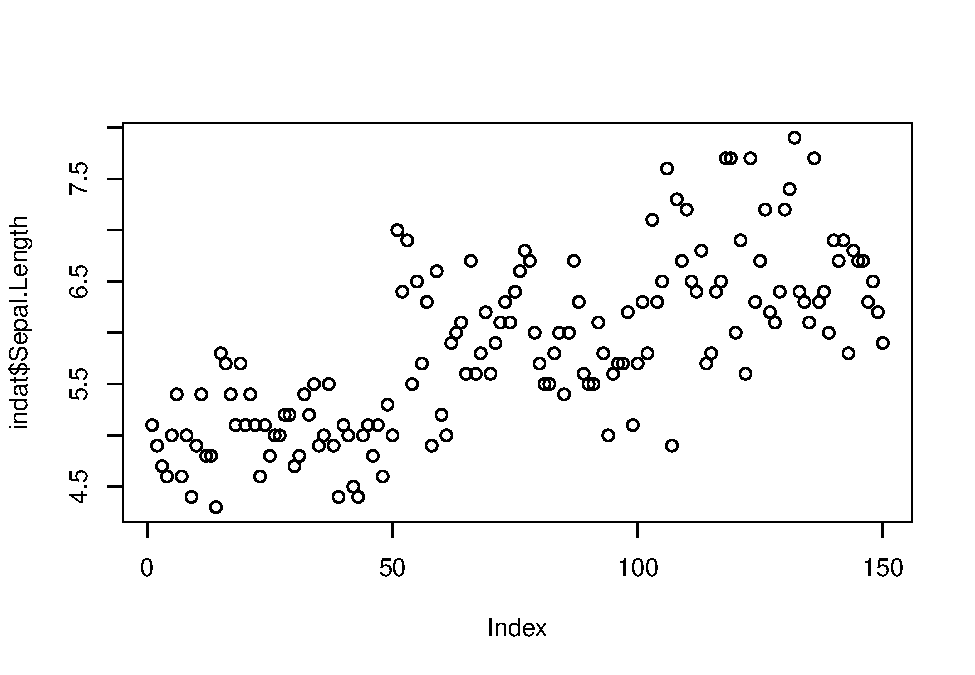
\includegraphics{TAMsIntro2RviaRStudioTutorial_files/figure-latex/unnamed-chunk-48-1.pdf}

In the following example, R evaluates the class of one of the arguments
as being a factor and hence tries to give you a sensible result, which
is producing a boxplot of a numerical variable as a function of a
factor.

\begin{Shaded}
\begin{Highlighting}[]
\NormalTok{ys}\OtherTok{\textless{}{-}}\NormalTok{indat}\SpecialCharTok{$}\NormalTok{Sepal.Length}
\NormalTok{xs}\OtherTok{\textless{}{-}}\NormalTok{indat}\SpecialCharTok{$}\NormalTok{Species}
\CommentTok{\#note use of \textasciitilde{} to represent "as a function of"}
\FunctionTok{plot}\NormalTok{(ys}\SpecialCharTok{\textasciitilde{}}\FunctionTok{as.factor}\NormalTok{(xs))}
\end{Highlighting}
\end{Shaded}

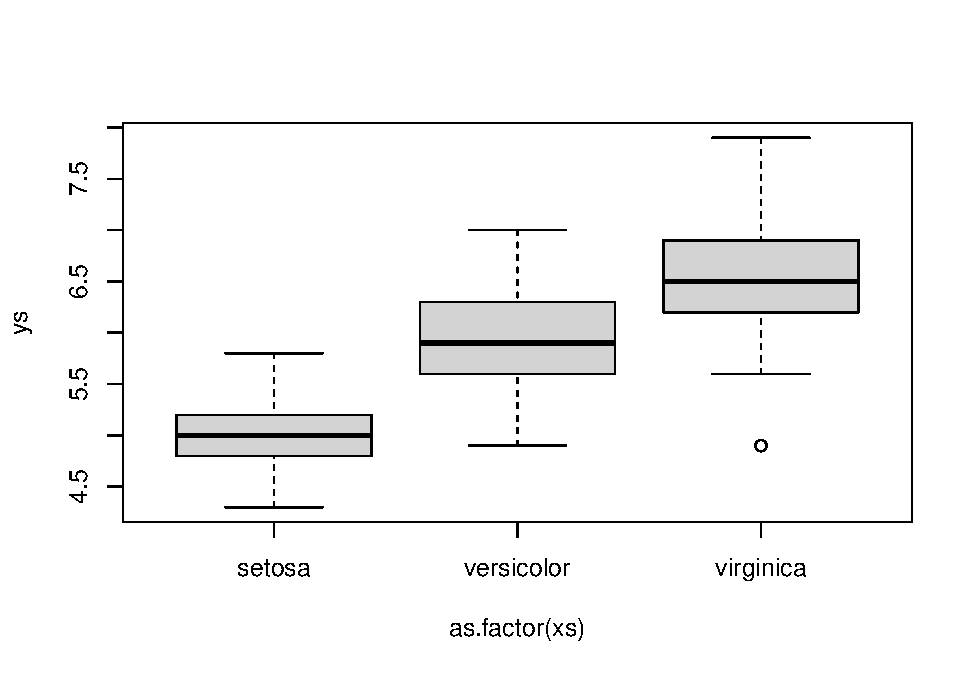
\includegraphics{TAMsIntro2RviaRStudioTutorial_files/figure-latex/unnamed-chunk-49-1.pdf}

Note the use of \texttt{\textasciitilde{}} to mean ``as a function of'';
this is also used below when specifying regression models, where the
object on the left of \texttt{\textasciitilde{}} will be the response
variable and the objects on the right explanatory variables.

We now add some labels to a new plot, using directly function
\texttt{boxplot} (which in the background \texttt{plot} above called),
of sepal length as a function of species

\begin{Shaded}
\begin{Highlighting}[]
\NormalTok{ys}\OtherTok{\textless{}{-}}\NormalTok{indat}\SpecialCharTok{$}\NormalTok{Sepal.Length}
\NormalTok{xs}\OtherTok{\textless{}{-}}\NormalTok{indat}\SpecialCharTok{$}\NormalTok{Species}
\CommentTok{\#note use of \textasciitilde{} to represent "as a function of"}
\FunctionTok{boxplot}\NormalTok{(ys}\SpecialCharTok{\textasciitilde{}}\NormalTok{xs,}\AttributeTok{ylab=}\StringTok{"Sepal Length (in mm)"}\NormalTok{,}\AttributeTok{main=}\StringTok{"Sepal length by species"}\NormalTok{)}
\end{Highlighting}
\end{Shaded}

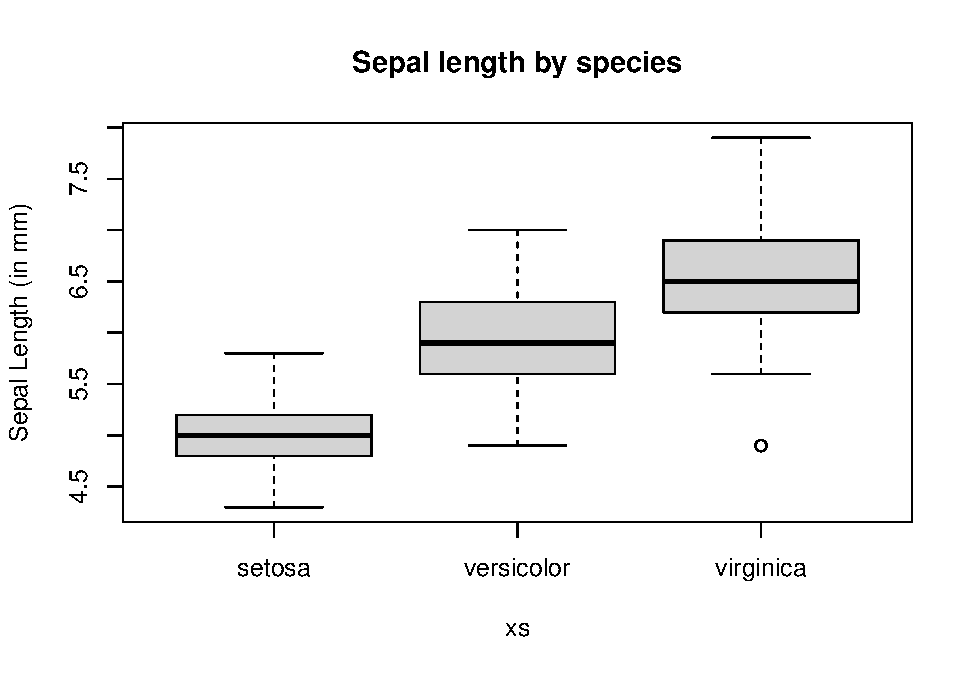
\includegraphics{TAMsIntro2RviaRStudioTutorial_files/figure-latex/unnamed-chunk-50-1.pdf}

\begin{Shaded}
\begin{Highlighting}[]
\CommentTok{\#compare with this code {-} next line returns an error}
\CommentTok{\#plot(ys\textasciitilde{}xs,ylab="Sepal Length (in mm)",main="Sepal length by species")}
\CommentTok{\#making species be a factor {-} allows the plot below to work well}
\CommentTok{\#xs\textless{}{-}as.factor(indat$Species)}
\CommentTok{\#plot(ys\textasciitilde{}xs,ylab="Sepal Length (in mm)",main="Sepal length by species")}
\end{Highlighting}
\end{Shaded}

We can also set the graphic window to hold multiple plots. This is
obtained via argument \texttt{mfrow}, one of the arguments in function.
Note this function controls a much larger number of graphical
parameters. You can take a look at its help file to get a feel for how
many and what kind of control it allows you. An example follows, in
which we leverage on the use of function \texttt{with} to avoid having
to constantly use \texttt{indat\$} to tell R where the data can be
found.

\begin{Shaded}
\begin{Highlighting}[]
\CommentTok{\#define 3 rows and 2 columns of plots}
\FunctionTok{par}\NormalTok{(}\AttributeTok{mfrow=}\FunctionTok{c}\NormalTok{(}\DecValTok{3}\NormalTok{,}\DecValTok{2}\NormalTok{))}
\FunctionTok{with}\NormalTok{(indat,}\FunctionTok{hist}\NormalTok{(Sepal.Length,}\AttributeTok{main=}\StringTok{""}\NormalTok{))}
\FunctionTok{with}\NormalTok{(indat,}\FunctionTok{hist}\NormalTok{(Sepal.Width,}\AttributeTok{main=}\StringTok{""}\NormalTok{))}
\FunctionTok{with}\NormalTok{(indat,}\FunctionTok{hist}\NormalTok{(Petal.Length,}\AttributeTok{main=}\StringTok{""}\NormalTok{))}
\FunctionTok{with}\NormalTok{(indat,}\FunctionTok{hist}\NormalTok{(Petal.Width,}\AttributeTok{main=}\StringTok{""}\NormalTok{))}
\FunctionTok{with}\NormalTok{(indat,}\FunctionTok{plot}\NormalTok{(Petal.Length,Petal.Width,}\AttributeTok{pch=}\DecValTok{21}\NormalTok{,}\AttributeTok{col=}\DecValTok{12}\NormalTok{,}\AttributeTok{bg=}\DecValTok{3}\NormalTok{))}
\FunctionTok{with}\NormalTok{(indat,}\FunctionTok{plot}\NormalTok{(Sepal.Length,Sepal.Width,}\AttributeTok{pch=}\DecValTok{16}\NormalTok{,}\AttributeTok{col=}\DecValTok{3}\NormalTok{))}
\end{Highlighting}
\end{Shaded}

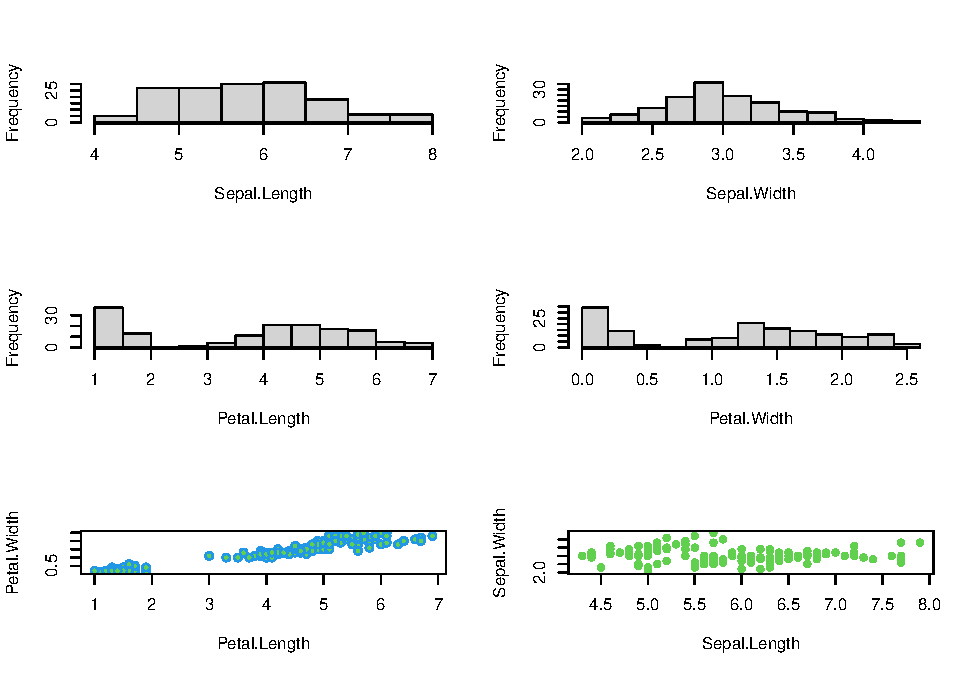
\includegraphics{TAMsIntro2RviaRStudioTutorial_files/figure-latex/unnamed-chunk-51-1.pdf}

We used argument \texttt{mfrow}, but looking at the help for function
\texttt{par} gives you an insight to the level of customization one can
reach with respect to these graphical parameters, via dozens of
different arguments.

We can look at the correlation structure between all variables using
function \texttt{pairs}.

\begin{Shaded}
\begin{Highlighting}[]
\CommentTok{\#note selection of just the first 4 columns, since the last is not numeric}
\FunctionTok{pairs}\NormalTok{(indat[,}\DecValTok{1}\SpecialCharTok{:}\DecValTok{4}\NormalTok{])}
\end{Highlighting}
\end{Shaded}

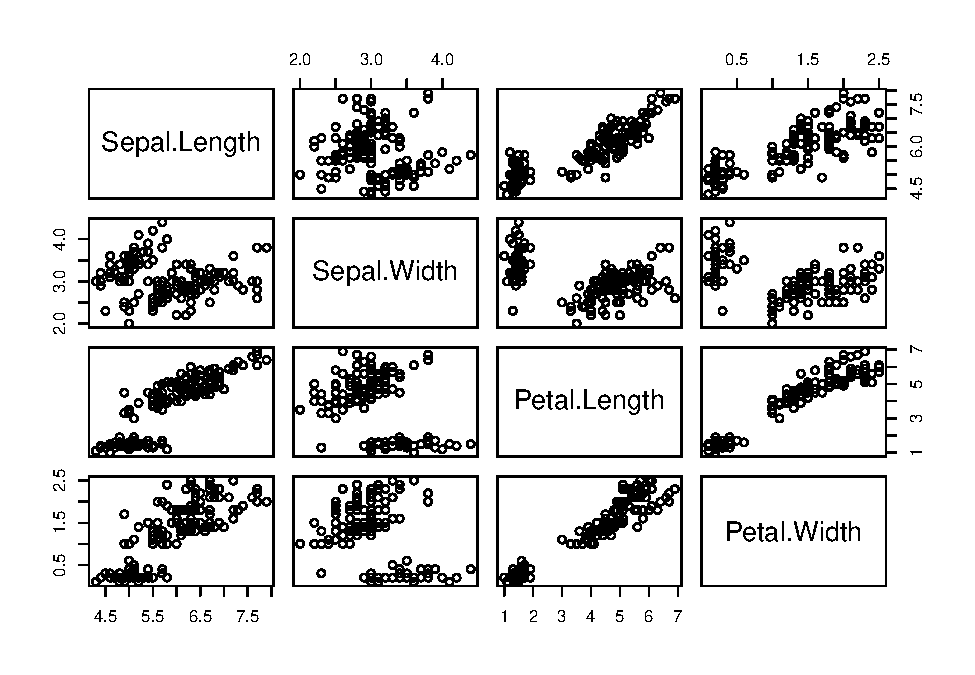
\includegraphics{TAMsIntro2RviaRStudioTutorial_files/figure-latex/unnamed-chunk-52-1.pdf}

\textbf{Task 3}: Using data \texttt{cars}, create a plot that represents
the stopping distances as a function of the speed of cars. Use the
\texttt{points} function to add a special symbol to points corresponding
to cars with speed lower than 15 mph, but distance larger than 70m.
Check out the function \texttt{text} to add text annotations to plots.
Customize axis labels.

Note that we can control most, if not all, elements of a plot. As an
example, see the following code, where I am controlling all sorts of
aspects. Search the help file to understand what the arguments
\texttt{mar} of function \texttt{par} does (sets margin sizes) as well
as \texttt{plot}'s parameters \texttt{xlim}, \texttt{ylim} \texttt{cex},
\texttt{pch}, \texttt{col}, do. See \texttt{?par} to check all the
graphical parameters you can control on plots.

\begin{Shaded}
\begin{Highlighting}[]
\FunctionTok{set.seed}\NormalTok{(}\DecValTok{1234}\NormalTok{)}
\FunctionTok{par}\NormalTok{(}\AttributeTok{mfrow=}\FunctionTok{c}\NormalTok{(}\DecValTok{1}\NormalTok{,}\DecValTok{3}\NormalTok{),}\AttributeTok{mar=}\FunctionTok{c}\NormalTok{(}\DecValTok{8}\NormalTok{,}\DecValTok{4}\NormalTok{,}\FloatTok{0.5}\NormalTok{,}\FloatTok{0.5}\NormalTok{))}
\NormalTok{pesos}\OtherTok{\textless{}{-}}\FunctionTok{rnorm}\NormalTok{(}\DecValTok{100}\NormalTok{,}\DecValTok{200}\NormalTok{,}\DecValTok{20}\NormalTok{)}
\NormalTok{sps}\OtherTok{\textless{}{-}}\FunctionTok{rep}\NormalTok{(}\FunctionTok{c}\NormalTok{(}\StringTok{"Carapau"}\NormalTok{,}\StringTok{"Sardinha"}\NormalTok{),}\AttributeTok{each=}\DecValTok{50}\NormalTok{)}
\FunctionTok{boxplot}\NormalTok{(pesos}\SpecialCharTok{\textasciitilde{}}\NormalTok{sps,}\AttributeTok{xlab=}\StringTok{"Espécie"}\NormalTok{,}\AttributeTok{ylab=}\StringTok{"Peso"}\NormalTok{,}\AttributeTok{las=}\DecValTok{1}\NormalTok{)}
\FunctionTok{boxplot}\NormalTok{(pesos}\SpecialCharTok{\textasciitilde{}}\NormalTok{sps,}\AttributeTok{xlab=}\StringTok{"Espécie"}\NormalTok{,}\AttributeTok{ylab=}\StringTok{"Peso"}\NormalTok{,}\AttributeTok{las=}\DecValTok{2}\NormalTok{,}\AttributeTok{col=}\DecValTok{3}\NormalTok{)}
\FunctionTok{plot}\NormalTok{(}\FunctionTok{rnorm}\NormalTok{(}\DecValTok{10}\NormalTok{),}\FunctionTok{rnorm}\NormalTok{(}\DecValTok{10}\NormalTok{),}\AttributeTok{xlim=}\FunctionTok{c}\NormalTok{(}\SpecialCharTok{{-}}\DecValTok{3}\NormalTok{,}\DecValTok{3}\NormalTok{),}\AttributeTok{ylim=}\FunctionTok{c}\NormalTok{(}\SpecialCharTok{{-}}\DecValTok{3}\NormalTok{,}\DecValTok{3}\NormalTok{),}\AttributeTok{col=}\StringTok{"blue"}\NormalTok{,}\AttributeTok{cex=}\DecValTok{2}\NormalTok{)}
\FunctionTok{points}\NormalTok{(}\FunctionTok{rnorm}\NormalTok{(}\DecValTok{10}\NormalTok{),}\FunctionTok{rnorm}\NormalTok{(}\DecValTok{10}\NormalTok{),}\AttributeTok{col=}\DecValTok{6}\NormalTok{,}\AttributeTok{cex=}\DecValTok{2}\NormalTok{,}\AttributeTok{pch=}\DecValTok{2}\NormalTok{)}
\FunctionTok{points}\NormalTok{(}\FunctionTok{rnorm}\NormalTok{(}\DecValTok{10}\NormalTok{),}\FunctionTok{rnorm}\NormalTok{(}\DecValTok{10}\NormalTok{),}\AttributeTok{col=}\StringTok{"orange"}\NormalTok{,}\AttributeTok{cex=}\DecValTok{4}\NormalTok{,}\AttributeTok{pch=}\DecValTok{17}\NormalTok{)}
\FunctionTok{points}\NormalTok{(}\FunctionTok{rnorm}\NormalTok{(}\DecValTok{10}\NormalTok{),}\FunctionTok{rnorm}\NormalTok{(}\DecValTok{10}\NormalTok{),}\AttributeTok{col=}\StringTok{"blue"}\NormalTok{,}\AttributeTok{cex=}\DecValTok{3}\NormalTok{,}\AttributeTok{pch=}\DecValTok{21}\NormalTok{,}\AttributeTok{bg=}\StringTok{"green"}\NormalTok{)}
\end{Highlighting}
\end{Shaded}

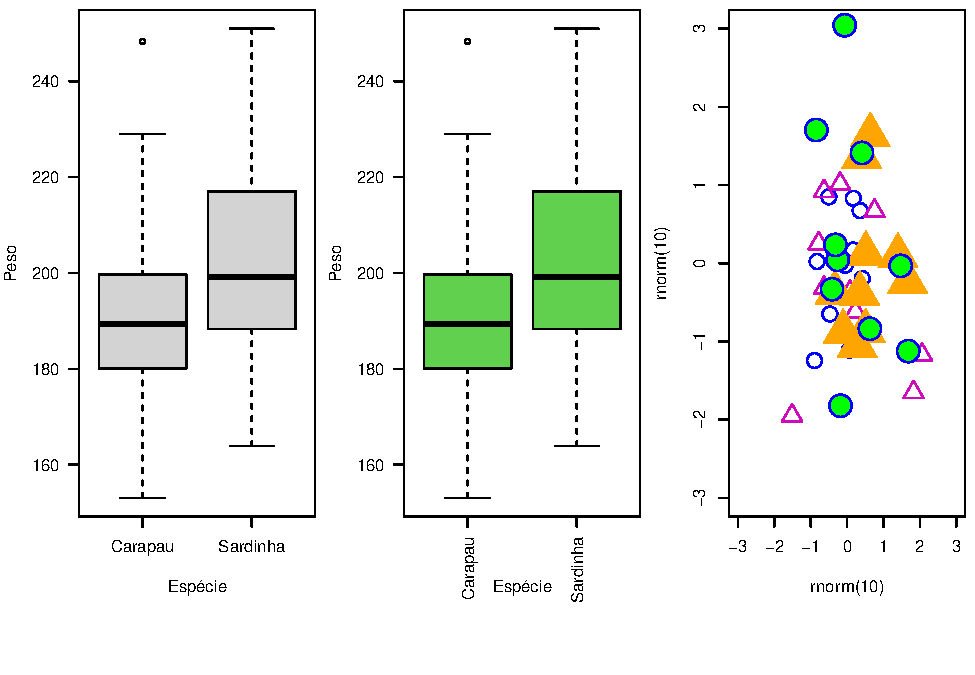
\includegraphics{TAMsIntro2RviaRStudioTutorial_files/figure-latex/unnamed-chunk-53-1.pdf}

Here and in class I will generally use R base for plots, but nowdays the
cool kids tend to use the ggplot2 system
(\url{https://r-graph-gallery.com/ggplot2-package.html}). It is worth to
go and find out about it.

If you really want to get creative with your plots, and a great plot can
be extremely useful in conveying a message, check out the gallery here:
\url{https://r-graph-gallery.com/} Lots of ideas, with the R code to use
them with your data!

\section{Extending basic capabilities via
packages}\label{extending-basic-capabilities-via-packages}

While R base installation includes enough functions that getting
acquainted with them could take several years, many more are available
via the installation of additional packages available online. A package
is just a set of functions and data sets (and the corresponding
documentation plus some additional required files) which usually have
some specific goal. As examples, in our course we will be using packages
\texttt{vegan} and \texttt{mgcv}, which allow the implementation of a
variety of numerical ecology techniques and generalized additive models
(GAM), respectively.

Note packages cover a very wide range of applications, and chances are
that at least a package, often more than one, already exists to
implement most kinds of statistical or data processing tasks we might
imagine.

Installing a new package in R requires a call to function
\texttt{install.packages}. A RStudio shortcut is simply to follow the
\texttt{Tools\textbar{}Install\ packages...} shortcut.

After a package is installed it needs to be loaded to be available. In R
this is done calling function \texttt{library} with the package name as
an argument. In RStudio this becomes simpler by checking the boxes under
the RStudio tab packages (by default this tab is available on the bottom
right window, along with the Files, Plots, Help and Viewer tabs).

We use \texttt{vegan} as an example. Notice to begin with that
\texttt{vegan} is not available yet

\begin{Shaded}
\begin{Highlighting}[]
\CommentTok{\#}
\NormalTok{?vegan}
\end{Highlighting}
\end{Shaded}

Next, we install the package.

\begin{Shaded}
\begin{Highlighting}[]
\CommentTok{\#}
\FunctionTok{install.packages}\NormalTok{(}\StringTok{"vegan"}\NormalTok{)}
\end{Highlighting}
\end{Shaded}

(note: do not install packages within a dynamic report, that would be a
akin to installing Word everytime you wanted to work on a document!)

Then, we load the package

\begin{Shaded}
\begin{Highlighting}[]
\CommentTok{\#}
\FunctionTok{library}\NormalTok{(}\StringTok{"vegan"}\NormalTok{)}
\end{Highlighting}
\end{Shaded}

\begin{verbatim}
## Loading required package: permute
\end{verbatim}

\begin{verbatim}
## Loading required package: lattice
\end{verbatim}

\begin{verbatim}
## This is vegan 2.6-8
\end{verbatim}

and finally we check that the functions in it are now loaded

\begin{Shaded}
\begin{Highlighting}[]
\CommentTok{\#}
\NormalTok{?vegan}
\end{Highlighting}
\end{Shaded}

We would now be ready to do all sorts of classification and ordination
techniques, say.

\textbf{Task 4}: Run the example code available in the help page from
the function \texttt{cca}. Try to understand what is happening.

\begin{Shaded}
\begin{Highlighting}[]
\CommentTok{\#here are the relevant lines of code to run}
\FunctionTok{data}\NormalTok{(varespec)}
\FunctionTok{data}\NormalTok{(varechem)}
\DocumentationTok{\#\# Common but bad way: use all variables you happen to have in your}
\DocumentationTok{\#\# environmental data matrix}
\NormalTok{vare.cca }\OtherTok{\textless{}{-}} \FunctionTok{cca}\NormalTok{(varespec, varechem)}
\NormalTok{vare.cca}
\FunctionTok{plot}\NormalTok{(vare.cca)}
\end{Highlighting}
\end{Shaded}

\section{Analysis example:
regression}\label{analysis-example-regression}

One of the most common type of data analysis is a regression model.
Despite common and conceptually simple, it is a very powerful way to
understand which (and how) of a number of candidate variables, sometimes
referred to covariates, independent or explanatory variables, might
influence a dependent variable, also often referred as the response.
There are many flavors of regression models, from a simple linear
regression to complicated generalized additive mixed models. We do not
wish to present these in any detail, but to introduce you to some
functions that implement these models and the syntax that R uses to
describe them.

Let's start with the basics. You have used the \texttt{cars} data set
above. We use it here again to try to explain the distance a car takes
to stop as a function of its speed. We start with a linear model using
function \texttt{lm}.

\begin{Shaded}
\begin{Highlighting}[]
\FunctionTok{data}\NormalTok{(cars)}
\NormalTok{mylm1}\OtherTok{\textless{}{-}}\FunctionTok{lm}\NormalTok{(dist}\SpecialCharTok{\textasciitilde{}}\NormalTok{speed,}\AttributeTok{data=}\NormalTok{cars)}
\end{Highlighting}
\end{Shaded}

We have stored the result of fitting the model in object \texttt{mylm1}.
The function \texttt{summary} can be used to print a summary of the fit

\begin{Shaded}
\begin{Highlighting}[]
\FunctionTok{summary}\NormalTok{(mylm1)}
\end{Highlighting}
\end{Shaded}

\begin{verbatim}
## 
## Call:
## lm(formula = dist ~ speed, data = cars)
## 
## Residuals:
##     Min      1Q  Median      3Q     Max 
## -29.069  -9.525  -2.272   9.215  43.201 
## 
## Coefficients:
##             Estimate Std. Error t value Pr(>|t|)    
## (Intercept) -17.5791     6.7584  -2.601   0.0123 *  
## speed         3.9324     0.4155   9.464 1.49e-12 ***
## ---
## Signif. codes:  0 '***' 0.001 '**' 0.01 '*' 0.05 '.' 0.1 ' ' 1
## 
## Residual standard error: 15.38 on 48 degrees of freedom
## Multiple R-squared:  0.6511, Adjusted R-squared:  0.6438 
## F-statistic: 89.57 on 1 and 48 DF,  p-value: 1.49e-12
\end{verbatim}

Do not get frightened about all the output. The coefficient associated
with speed tells us what intuition alone would anticipate, the higher
the speed, the larger the distance a car takes to stop. The easier way
to see the relationship is by adding a line to the plot (note this is a
similar plot to what you should have created in task 3 above!). The
predicted relationship is shown next:

\begin{Shaded}
\begin{Highlighting}[]
\NormalTok{xl}\OtherTok{\textless{}{-}}\StringTok{"Speed (mph)"}
\NormalTok{yl}\OtherTok{\textless{}{-}}\StringTok{"Distance (m)"}
\FunctionTok{plot}\NormalTok{(cars}\SpecialCharTok{$}\NormalTok{speed,cars}\SpecialCharTok{$}\NormalTok{dist,}\AttributeTok{xlab=}\NormalTok{xl,}\AttributeTok{ylab=}\NormalTok{yl,}\AttributeTok{ylim=}\FunctionTok{c}\NormalTok{(}\DecValTok{0}\NormalTok{,}\DecValTok{120}\NormalTok{),}\AttributeTok{xlim=}\FunctionTok{c}\NormalTok{(}\DecValTok{0}\NormalTok{,}\DecValTok{30}\NormalTok{))}
\FunctionTok{abline}\NormalTok{(mylm1)}
\end{Highlighting}
\end{Shaded}

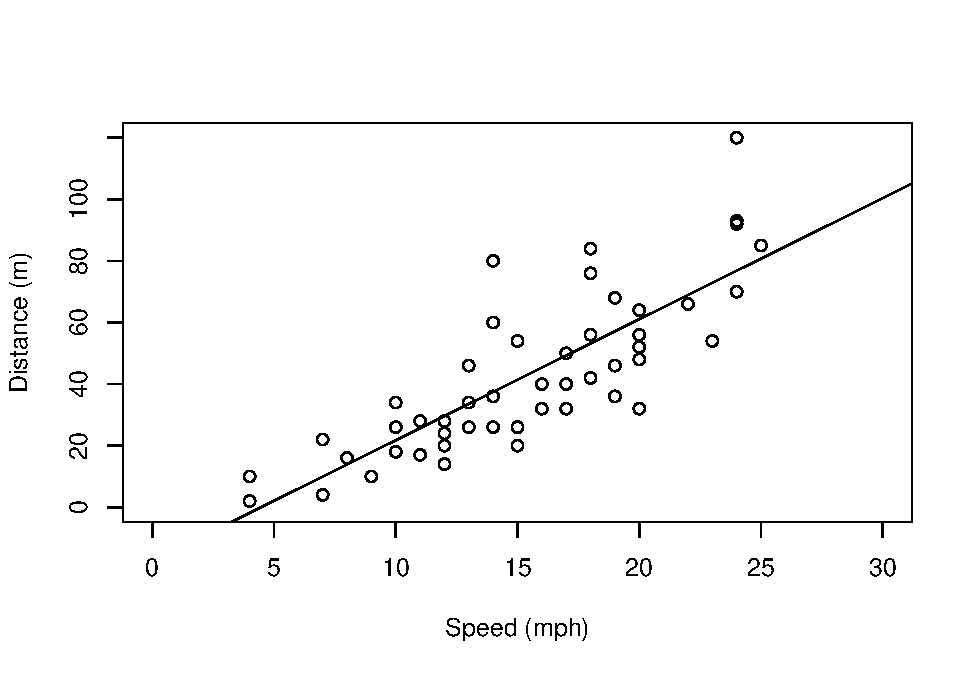
\includegraphics{TAMsIntro2RviaRStudioTutorial_files/figure-latex/chunck159-1.pdf}

Note how function \texttt{abline} is used with a linear model as its
first argument and it uses the parameters in said object to add a line
to the plot. The optional arguments \texttt{v} and \texttt{h} are often
very useful to draw vertical and horizontal lines in plots.

\textbf{Task 5}: Use abline to draw dashed lines (tip, use optional
argument \texttt{lty}=2) representing the estimated distance that a car
moving at 16 mph would take to stop.

Note that the line added to the plot represents the distance a car would
take to stop given its speed. Oddly enough, it seems like a car going at
3 mph might take a negative time to stop, which is just plain nonsense.
Why? Because we used a model which does not respect the features of the
data. A stopping distance can't be negative! However, implicit in the
linear model we used, distance is a Gaussian (=normal) random variable.
We can avoid this by using a generalized linear model (GLM). Now the
response can have a range of distributions. An example of such
distribution that takes only positive values is the gamma distribution.
We implement a gamma GLM next

\begin{Shaded}
\begin{Highlighting}[]
\CommentTok{\#fit the GLM}
\NormalTok{myglm1}\OtherTok{\textless{}{-}}\FunctionTok{glm}\NormalTok{(dist}\SpecialCharTok{\textasciitilde{}}\NormalTok{speed,}\AttributeTok{data=}\NormalTok{cars,}\AttributeTok{family=}\FunctionTok{Gamma}\NormalTok{(}\AttributeTok{link=}\NormalTok{log))}
\CommentTok{\#predict using the GLM for speeds between 1 and 30}
\NormalTok{predmyglm1}\OtherTok{\textless{}{-}}\FunctionTok{predict.glm}\NormalTok{(myglm1,}
\AttributeTok{newdata=}\FunctionTok{data.frame}\NormalTok{(}\AttributeTok{speed=}\DecValTok{1}\SpecialCharTok{:}\DecValTok{30}\NormalTok{),}\AttributeTok{type=}\StringTok{"response"}\NormalTok{)}
\end{Highlighting}
\end{Shaded}

Our model now assumes the response has a gamma distribution, and the
link function is the logarithm. The link function allows you to change
how the mean value is related to the covariates. This becomes rather
technical rather fast. Details about GLMs are naturally beyond the scope
of this tutorial. References like Faraway (2006) or Zuur \emph{et al.}
(2009) will provide further details in an applied context. The predicted
relationship is shown in the next figure.

\begin{Shaded}
\begin{Highlighting}[]
\CommentTok{\#create a plot}
\FunctionTok{plot}\NormalTok{(cars}\SpecialCharTok{$}\NormalTok{speed,cars}\SpecialCharTok{$}\NormalTok{dist,}\AttributeTok{xlab=}\StringTok{"Speed (mph)"}\NormalTok{,}
\AttributeTok{ylab=}\StringTok{"Distance (m)"}\NormalTok{,}\AttributeTok{ylim=}\FunctionTok{c}\NormalTok{(}\DecValTok{0}\NormalTok{,}\DecValTok{120}\NormalTok{),}\AttributeTok{xlim=}\FunctionTok{c}\NormalTok{(}\DecValTok{0}\NormalTok{,}\DecValTok{30}\NormalTok{))}
\CommentTok{\#add the linear fit}
\FunctionTok{abline}\NormalTok{(mylm1)}
\CommentTok{\#and now add the glm predictions}
\FunctionTok{lines}\NormalTok{(}\DecValTok{1}\SpecialCharTok{:}\DecValTok{30}\NormalTok{,predmyglm1,}\AttributeTok{col=}\StringTok{"blue"}\NormalTok{,}\AttributeTok{lwd=}\DecValTok{3}\NormalTok{,}\AttributeTok{lty=}\DecValTok{3}\NormalTok{)}
\end{Highlighting}
\end{Shaded}

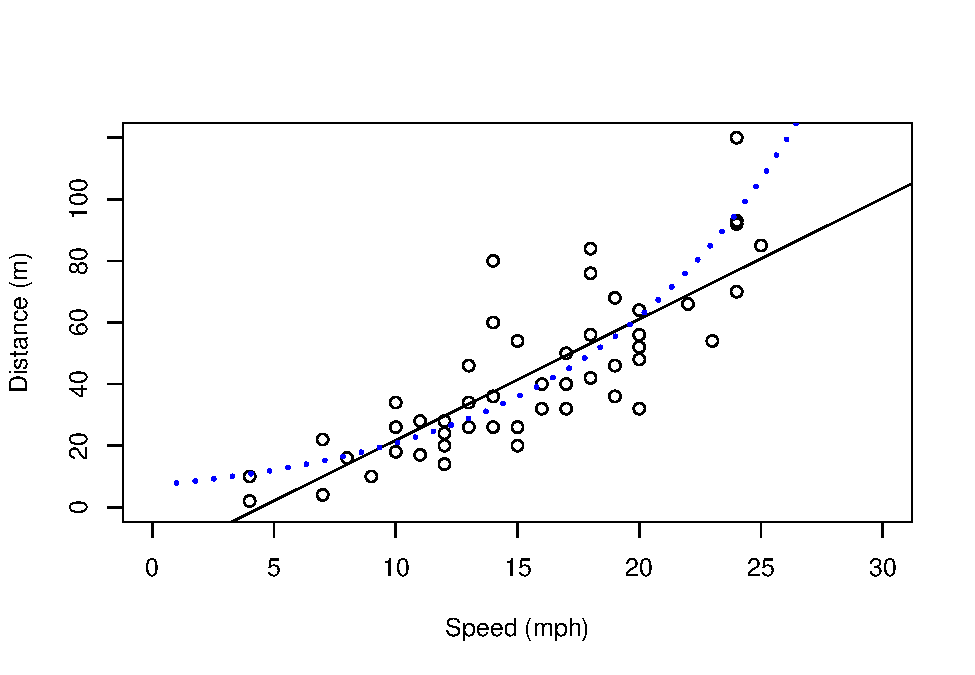
\includegraphics{TAMsIntro2RviaRStudioTutorial_files/figure-latex/unnamed-chunk-62-1.pdf}

However, this GLM still requires that the response is linear at some
scale (in this case, on the scale of the link function). Sometimes,
non-linear effects are present. These can be fitted using generalized
additive models. A good introduction to GAMs is provided by Wood (2006)
and Zuur \emph{et al.} (2009).

So finally we fit a GAM model to the same data set. For that we require
library \texttt{mgcv}. The outcome is shown below. Here the fit is not
very different from the GLM fit, but under many circumstances a GAM
might be required over a GLM. We will see such an example in the next
few days, when we model the detectability of beaked whale clicks as a
function of distance and angle (with respect to hydrophones).

\begin{Shaded}
\begin{Highlighting}[]
\CommentTok{\#load the mgcv library}
\FunctionTok{library}\NormalTok{(mgcv)}
\end{Highlighting}
\end{Shaded}

\begin{verbatim}
## Loading required package: nlme
\end{verbatim}

\begin{verbatim}
## This is mgcv 1.9-1. For overview type 'help("mgcv-package")'.
\end{verbatim}

\begin{Shaded}
\begin{Highlighting}[]
\CommentTok{\#fit the GAM}
\NormalTok{mygam1}\OtherTok{\textless{}{-}}\FunctionTok{gam}\NormalTok{(dist}\SpecialCharTok{\textasciitilde{}}\FunctionTok{s}\NormalTok{(speed),}\AttributeTok{data=}\NormalTok{cars,}\AttributeTok{family=}\FunctionTok{Gamma}\NormalTok{(}\AttributeTok{link=}\NormalTok{log))}
\CommentTok{\#predict using the GAM for speeds between 1 and 30}
\NormalTok{predmygam1}\OtherTok{\textless{}{-}}\FunctionTok{predict}\NormalTok{(mygam1,}\AttributeTok{newdata=}\FunctionTok{data.frame}\NormalTok{(}\AttributeTok{speed=}\DecValTok{1}\SpecialCharTok{:}\DecValTok{30}\NormalTok{),}
\AttributeTok{type=}\StringTok{"response"}\NormalTok{)}
\end{Highlighting}
\end{Shaded}

\begin{Shaded}
\begin{Highlighting}[]
\CommentTok{\#create a plot}
\FunctionTok{plot}\NormalTok{(cars}\SpecialCharTok{$}\NormalTok{speed,cars}\SpecialCharTok{$}\NormalTok{dist,}\AttributeTok{xlab=}\StringTok{"Speed (mph)"}\NormalTok{,}
\AttributeTok{ylab=}\StringTok{"Distance (m)"}\NormalTok{,}\AttributeTok{ylim=}\FunctionTok{c}\NormalTok{(}\DecValTok{0}\NormalTok{,}\DecValTok{120}\NormalTok{),}\AttributeTok{xlim=}\FunctionTok{c}\NormalTok{(}\DecValTok{0}\NormalTok{,}\DecValTok{30}\NormalTok{))}
\CommentTok{\#add the linear fit}
\FunctionTok{abline}\NormalTok{(mylm1)}
\CommentTok{\#and now add the GLM predictions}
\FunctionTok{lines}\NormalTok{(}\DecValTok{1}\SpecialCharTok{:}\DecValTok{30}\NormalTok{,predmyglm1,}\AttributeTok{col=}\StringTok{"blue"}\NormalTok{,}\AttributeTok{lwd=}\DecValTok{3}\NormalTok{,}\AttributeTok{lty=}\DecValTok{3}\NormalTok{)}
\FunctionTok{lines}\NormalTok{(}\DecValTok{1}\SpecialCharTok{:}\DecValTok{30}\NormalTok{,predmygam1,}\AttributeTok{col=}\StringTok{"green"}\NormalTok{,}\AttributeTok{lwd=}\DecValTok{3}\NormalTok{,}\AttributeTok{lty=}\DecValTok{2}\NormalTok{)}
\end{Highlighting}
\end{Shaded}

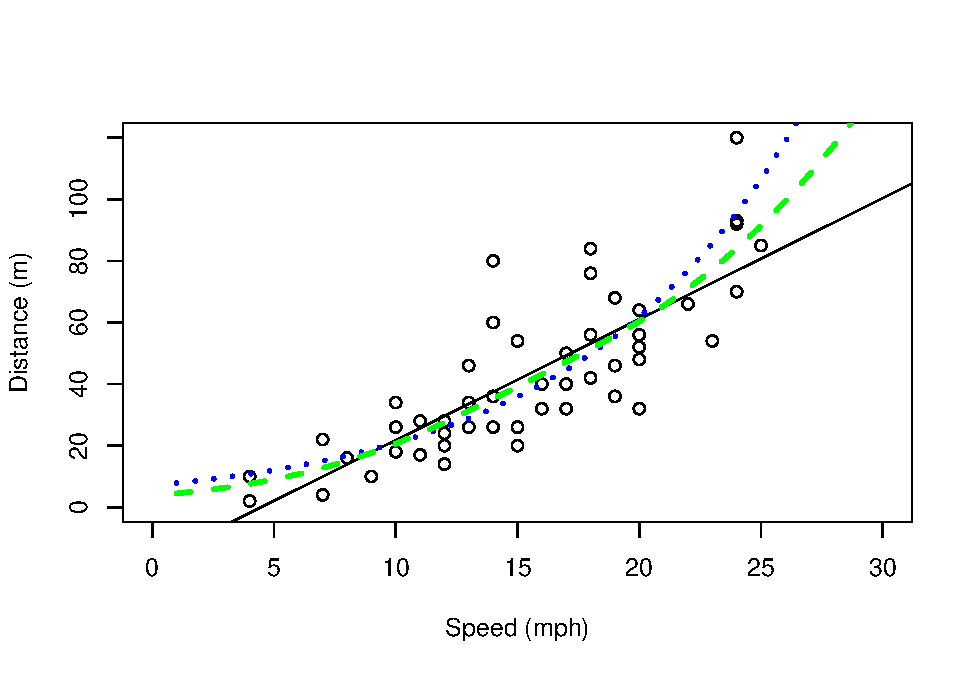
\includegraphics{TAMsIntro2RviaRStudioTutorial_files/figure-latex/unnamed-chunk-64-1.pdf}

\section{Simulation and random number
generation}\label{simulation-and-random-number-generation}

Another powerful use of R is for simulation. To this end, R has the
ability to simulate random deviates from a large number of
distributions. Perhaps the more useful and commonly used are the uniform
and the Gaussian distributions. We now create 50 random deviates from
each of these, as well as some Poisson deviates, for illustration

\begin{Shaded}
\begin{Highlighting}[]
\CommentTok{\#generate 50 pseudo{-}random Guassian numbers with mean 20 and standard deviation 3}
\NormalTok{rdnorm}\OtherTok{\textless{}{-}}\FunctionTok{rnorm}\NormalTok{(}\DecValTok{50}\NormalTok{,}\AttributeTok{mean=}\DecValTok{20}\NormalTok{,}\AttributeTok{sd=}\DecValTok{3}\NormalTok{)}
\CommentTok{\#generate 50 pseudo{-}random  50 uniform numbers between 3 and 6}
\NormalTok{rdunif}\OtherTok{\textless{}{-}}\FunctionTok{runif}\NormalTok{(}\DecValTok{50}\NormalTok{,}\AttributeTok{min=}\DecValTok{3}\NormalTok{,}\AttributeTok{max=}\DecValTok{6}\NormalTok{)}
\CommentTok{\#generate 50 pseudo{-}random  50 Poisson numbers with mean 6}
\NormalTok{rdpois}\OtherTok{\textless{}{-}}\FunctionTok{rpois}\NormalTok{(}\DecValTok{50}\NormalTok{,}\AttributeTok{lambda=}\DecValTok{6}\NormalTok{)}
\end{Highlighting}
\end{Shaded}

R can create random numbers from many different distributions (see
help(Distributions) for a list) -- the relevant functions generally
start with r and then an abbreviated distribution name (\texttt{rbinom},
\texttt{rexp}, \texttt{rgeom}, etc). Additionally, R also includes the
ability to obtain the density function, distribution function and
quantile function via the \texttt{d}+name, \texttt{p}+name and
\texttt{q}+name functions. As an example, the Gaussian function usage of
these functions is presented below

\begin{Shaded}
\begin{Highlighting}[]
\FunctionTok{dnorm}\NormalTok{(}\DecValTok{0}\NormalTok{,}\AttributeTok{mean=}\DecValTok{0}\NormalTok{,}\AttributeTok{sd=}\DecValTok{1}\NormalTok{)}
\end{Highlighting}
\end{Shaded}

\begin{verbatim}
## [1] 0.3989423
\end{verbatim}

\begin{Shaded}
\begin{Highlighting}[]
\FunctionTok{pnorm}\NormalTok{(}\DecValTok{0}\NormalTok{,}\AttributeTok{mean=}\DecValTok{0}\NormalTok{,}\AttributeTok{sd=}\DecValTok{1}\NormalTok{)}
\end{Highlighting}
\end{Shaded}

\begin{verbatim}
## [1] 0.5
\end{verbatim}

\begin{Shaded}
\begin{Highlighting}[]
\FunctionTok{qnorm}\NormalTok{(}\FloatTok{0.975}\NormalTok{,}\AttributeTok{mean=}\DecValTok{0}\NormalTok{,}\AttributeTok{sd=}\DecValTok{1}\NormalTok{)}
\end{Highlighting}
\end{Shaded}

\begin{verbatim}
## [1] 1.959964
\end{verbatim}

\textbf{Task 6}: Using what you have learnt here, create two histograms,
one of 50, another of 5000, random deviates from a Gaussian distribution
(you can choose the mean and standard deviation you prefer!), using the
optional argument \texttt{freq=FALSE} (leading to an estimate of the
density function). Then add a line to the plot that represents the true
underlying density (tip, you can use function \texttt{dnorm}), and
comment on the results. You can also do similar experiments with other
distributions. How weird are a beta(1,1), a beta(1,5) and a
beta(0.5,0.5) distributions (tip, you can use function \texttt{rbeta} or
\texttt{dbeta}). Can you guess which one is sometimes referred to as
bath tub distribution. What quantities do you imagine a beta might be
useful to model?

\section{Programming tricks}\label{programming-tricks}

Some very useful programming structures are those required to evaluate
conditional statements and those used to repeat statements many times.
These are fundamental for implementing simulations. In R we have
\texttt{if} statements and \texttt{for} loops, respectively.

As an example, see how an if statement works

\begin{Shaded}
\begin{Highlighting}[]
\NormalTok{X}\OtherTok{=}\DecValTok{2}
\ControlFlowTok{if}\NormalTok{ (X}\SpecialCharTok{\textgreater{}}\DecValTok{0}\NormalTok{) }\FunctionTok{print}\NormalTok{(X}\SpecialCharTok{+}\DecValTok{3}\NormalTok{)}
\end{Highlighting}
\end{Shaded}

\begin{verbatim}
## [1] 5
\end{verbatim}

One can also use an if-else statement, which executes either (1)
something or (2) something else, depending on the condition being TRUE
or FALSE. Here's an example:

\begin{Shaded}
\begin{Highlighting}[]
\NormalTok{X}\OtherTok{=}\DecValTok{2}
\ControlFlowTok{if}\NormalTok{ (X}\SpecialCharTok{\textgreater{}}\DecValTok{0}\NormalTok{)}
\NormalTok{  \{Y}\OtherTok{=}\FunctionTok{abs}\NormalTok{(X)\} }\ControlFlowTok{else} 
\NormalTok{  \{Y}\OtherTok{=}\NormalTok{X}\SpecialCharTok{\^{}}\DecValTok{2}\NormalTok{\}}
\NormalTok{Y}
\end{Highlighting}
\end{Shaded}

\begin{verbatim}
## [1] 2
\end{verbatim}

\begin{Shaded}
\begin{Highlighting}[]
\NormalTok{X}\OtherTok{=}\SpecialCharTok{{-}}\DecValTok{5}
\ControlFlowTok{if}\NormalTok{ (X}\SpecialCharTok{\textgreater{}}\DecValTok{0}\NormalTok{)}
\NormalTok{  \{Y}\OtherTok{=}\FunctionTok{abs}\NormalTok{(X)\} }\ControlFlowTok{else} 
\NormalTok{  \{Y}\OtherTok{=}\NormalTok{X}\SpecialCharTok{\^{}}\DecValTok{2}\NormalTok{\}}
\NormalTok{Y}
\end{Highlighting}
\end{Shaded}

\begin{verbatim}
## [1] 25
\end{verbatim}

on the other side, here's how a for loop works

\begin{Shaded}
\begin{Highlighting}[]
\NormalTok{n}\OtherTok{=}\DecValTok{4}
\NormalTok{X}\OtherTok{=}\DecValTok{1}\SpecialCharTok{:}\NormalTok{n}
\ControlFlowTok{for}\NormalTok{ (i }\ControlFlowTok{in} \DecValTok{1}\SpecialCharTok{:}\NormalTok{n) }\FunctionTok{print}\NormalTok{(i}\SpecialCharTok{+}\DecValTok{3}\NormalTok{)}
\end{Highlighting}
\end{Shaded}

\begin{verbatim}
## [1] 4
## [1] 5
## [1] 6
## [1] 7
\end{verbatim}

note there is nothing special about the use of i for an index; you can
use any index that you might want

\begin{Shaded}
\begin{Highlighting}[]
\NormalTok{n}\OtherTok{=}\DecValTok{4}
\NormalTok{X}\OtherTok{=}\DecValTok{1}\SpecialCharTok{:}\NormalTok{n}
\ControlFlowTok{for}\NormalTok{ (j }\ControlFlowTok{in} \DecValTok{1}\SpecialCharTok{:}\NormalTok{n) }\FunctionTok{print}\NormalTok{(}\FunctionTok{sum}\NormalTok{(}\FunctionTok{c}\NormalTok{(j,j}\SpecialCharTok{+}\DecValTok{3}\NormalTok{)))}
\end{Highlighting}
\end{Shaded}

\begin{verbatim}
## [1] 5
## [1] 7
## [1] 9
## [1] 11
\end{verbatim}

or even

\begin{Shaded}
\begin{Highlighting}[]
\NormalTok{n}\OtherTok{=}\DecValTok{4}
\NormalTok{X}\OtherTok{=}\DecValTok{1}\SpecialCharTok{:}\NormalTok{n}
\ControlFlowTok{for}\NormalTok{ (i }\ControlFlowTok{in}\NormalTok{ X) \{}
  \FunctionTok{cat}\NormalTok{(}\FunctionTok{paste}\NormalTok{(}\StringTok{"The i currently is:"}\NormalTok{,i),}\AttributeTok{sep=}\StringTok{"}\SpecialCharTok{\textbackslash{}n}\StringTok{"}\NormalTok{)}
  \FunctionTok{cat}\NormalTok{(}\FunctionTok{paste}\NormalTok{(}\StringTok{"The i+3 currently is:"}\NormalTok{,i}\SpecialCharTok{+}\DecValTok{3}\NormalTok{),}\AttributeTok{sep=}\StringTok{"}\SpecialCharTok{\textbackslash{}n}\StringTok{"}\NormalTok{)}
\NormalTok{  \}}
\end{Highlighting}
\end{Shaded}

\begin{verbatim}
## The i currently is: 1
## The i+3 currently is: 4
## The i currently is: 2
## The i+3 currently is: 5
## The i currently is: 3
## The i+3 currently is: 6
## The i currently is: 4
## The i+3 currently is: 7
\end{verbatim}

See above, explore R. Change the code. Repeat. Check for yourself what
\texttt{cat} and \texttt{paste} can be used for!

\textbf{Task 7}: Create 9 histograms of samples of Gaussian random
variables, adding the mean value on the plot as a vertical dashed line,
in blue if the mean of the observations is positive and in red if the
mean of the observations is negative.

Other interesting structures for ``control flow'' are the
\texttt{while}, \texttt{repeat} and \texttt{break}. Look into the help,
\texttt{?if}, to see details.

\section{Writing your own functions}\label{writing-your-own-functions}

While the above functions, and the many more available, make R a very
useful tool, there are sometimes problems which require a special tool.
For these, we can create our own functions. Note this is an advanced
topic.

The way of doing that follows a specific syntax

\texttt{\textgreater{}\ name\ \textless{}-\ function(arg1,arg2,...)\ \{what\ the\ function\ does\ goes\ here\}}

As an example, we create a function that returns the sum of its 2
arguments:

\begin{Shaded}
\begin{Highlighting}[]
\NormalTok{myfun}\OtherTok{\textless{}{-}}\ControlFlowTok{function}\NormalTok{(i,j)\{}
\NormalTok{  myres}\OtherTok{\textless{}{-}}\NormalTok{i}\SpecialCharTok{+}\NormalTok{j}
  \FunctionTok{return}\NormalTok{(myres)}
\NormalTok{\}}
\end{Highlighting}
\end{Shaded}

You can now see the function in the works

\begin{Shaded}
\begin{Highlighting}[]
\FunctionTok{myfun}\NormalTok{(}\DecValTok{3}\NormalTok{,}\DecValTok{5}\NormalTok{)}
\end{Highlighting}
\end{Shaded}

\begin{verbatim}
## [1] 8
\end{verbatim}

Note a function could have many arguments, none, or just one.

\textbf{Task 8}: create a function called \texttt{mystats} which returns
the mean, variance, maximum and minimum of the first, and only, argument
(a vector). Then, update your function such that it can also return the
mean excluding the negative numbers. Then, create some other function
you might think could be useful.

Creating your own functions will unleash strong R power, increasing
significantly your ability to manipulate, analyze and simulate data.

\section{Final tasks}\label{final-tasks}

These tasks are only intended for the students in Modelação Ecológica.
If you are a Ecologia Numérica student you can try it at your own risk!
If you are neither of those, then feel free to work through the material
regardless.

\subsection{A final task integrating all of the
above}\label{a-final-task-integrating-all-of-the-above}

Here we will implement an exercise were we pretend we are sampling an
animal population, using some (very basic) simulations to understand the
process better. Create plots that represent all the steps of your task,
with proper legends, labels, colors, etc, and add all your comments to
the dynamic report.

This exercise simulates a distance sampling survey. If you want to know
more about it, you can check this 2 page introduction paper on the topic
\href{https://github.com/TiagoAMarques/AnIntro2RTutorial/blob/40f353b63cb465c36dfa8f358e0e0d1cba45967a/Marques2009b.pdf}{here}.
It is one of the most often used methods to estimate the abundance
and/or density of wildlife populations.

\begin{enumerate}
\def\labelenumi{\arabic{enumi}.}
\item
  Simulate the positions of 10000 animals in a study area, with length
  10km and width 1km. Assume that any animal has an equal chance to be
  at any location in the study area (this corresponds to a uniform
  density surface).
\item
  Generate a transect at a random location along the study area.
\item
  Assume that you can potentially detect at most animals up to 500
  meters from your transect. Count all the animals that you would detect
  if detection was perfect across your transect.
\item
  Consider that animals far from your transect are harder to detect -
  yes, you are doing distance sampling! Define a function that
  represents a distance sampling half-normal detection function. If you
  do not know what that looks like check
  \href{https://workshops.distancesampling.org/online-course/lecturepdfs/Ch1/L1-4\%20Choosing\%20a\%20Detection\%20Function.pdf}{here},
  around slide 9. Assume that sigma=200m.
\item
  Simulate the detection process and get a sample of those animals
  detected. This is the hard bit, creating an animal detector. Tip:
  using \texttt{runif} will help. Ask me for details if you need them.
\item
  Create a plot that allows you to estimate (at this stage just a visual
  guess is needed) the detection probability.
\item
  Repeat the sampling process 500 times, and store the number of animals
  detected in each one of your simulated surveys.
\item
  plot the distribution of the number of animals that you would detect
  each new survey.
\end{enumerate}

Take your own conclusions about all that you did.

\subsection{Creating your own statistical test via
resampling}\label{creating-your-own-statistical-test-via-resampling}

\textbf{This is work in progress}

We are all used to implementing statistical tests. But statistical tests
for the situations one might face with real ecological data are not
always available. For that reason, it might be useful to know how to
create your own statistical tests. One can do that if one is able to
create a test statistic, that contains information about the hypothesis
one wishes to test, and for which we can simulate the distribution
assuming that the null hypothesis is true.

Let us consider an example where we have data from camera traps, and we
want to see if there is some relationship between two species. In
particular, we want to see if the use of the area covered by the camera
is dependent on what species were present there before.

Imagine we have a camera trap and we collect the order in which
different species appeared on the camera.

\begin{Shaded}
\begin{Highlighting}[]
\CommentTok{\#the exercise is more interesting if you do not think about how the data is being created}
\CommentTok{\#later you can look at it, but for now, just treat this as a black box}
\CommentTok{\#so all get the same answers}
\FunctionTok{set.seed}\NormalTok{(}\DecValTok{189}\NormalTok{)}
\NormalTok{species}\OtherTok{\textless{}{-}}\FunctionTok{c}\NormalTok{(}\StringTok{"wolf"}\NormalTok{,}\StringTok{"bear"}\NormalTok{,}\StringTok{"deer"}\NormalTok{,}\StringTok{"racoon"}\NormalTok{,}\StringTok{"weasel"}\NormalTok{,}\StringTok{"bobcat"}\NormalTok{,}\StringTok{"badger"}\NormalTok{,}\StringTok{"squirel"}\NormalTok{,}\StringTok{"sheep"}\NormalTok{)}
\NormalTok{abundances}\OtherTok{\textless{}{-}}\FunctionTok{c}\NormalTok{(}\DecValTok{50}\NormalTok{,}\DecValTok{20}\NormalTok{,}\DecValTok{300}\NormalTok{,}\DecValTok{500}\NormalTok{,}\DecValTok{500}\NormalTok{,}\DecValTok{50}\NormalTok{,}\DecValTok{400}\NormalTok{,}\DecValTok{1000}\NormalTok{,}\DecValTok{200}\NormalTok{)}
\NormalTok{appearences}\OtherTok{\textless{}{-}}\FunctionTok{rep}\NormalTok{(species,}\AttributeTok{times=}\NormalTok{abundances)}
\NormalTok{n}\OtherTok{\textless{}{-}}\FunctionTok{length}\NormalTok{(appearences)}
\NormalTok{appearences}\OtherTok{\textless{}{-}}\NormalTok{appearences[}\FunctionTok{sample}\NormalTok{(}\DecValTok{1}\SpecialCharTok{:}\NormalTok{n,}\AttributeTok{size =}\NormalTok{ n,}\AttributeTok{replace=}\ConstantTok{FALSE}\NormalTok{)]}
\end{Highlighting}
\end{Shaded}

The code above has simulated such data, creating 3020 sequential
occurrences of 9 different species. Here's the number of observations
per species

\begin{Shaded}
\begin{Highlighting}[]
\FunctionTok{barplot}\NormalTok{(}\FunctionTok{table}\NormalTok{(appearences))}
\end{Highlighting}
\end{Shaded}

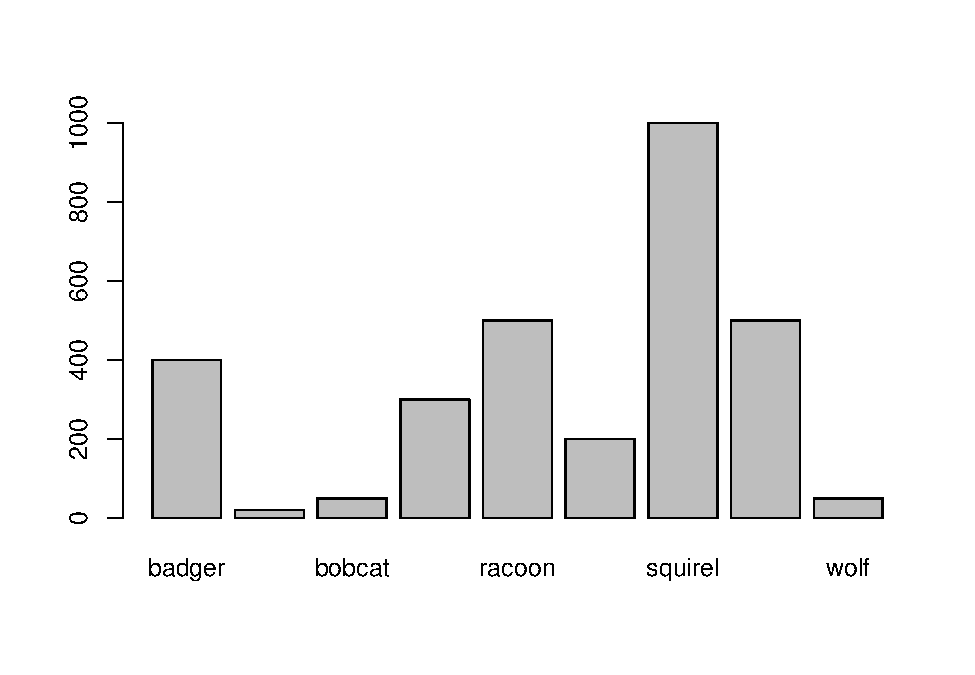
\includegraphics{TAMsIntro2RviaRStudioTutorial_files/figure-latex/unnamed-chunk-75-1.pdf}

We can see the first few detections

\begin{Shaded}
\begin{Highlighting}[]
\FunctionTok{head}\NormalTok{(appearences)}
\end{Highlighting}
\end{Shaded}

\begin{verbatim}
## [1] "weasel"  "squirel" "badger"  "racoon"  "squirel" "sheep"
\end{verbatim}

Recent research indicates that squirels tend to appear after weasels
appear, and you have been tasked with looking into the data to test
whether that seems to be the case at this site. How can you do it?

You will immediately realize this puts you in a context that you have
not learnt any statistical significance tests that sound useful here.
You need to create your own test. This can be done as a
resampling/permutation test.

You first define a null hypothesis. That could be

H0: the appearance of a squirrel does not depend on badgers having been
present

Next, you need to get a test statistic. It seems like a good test
statistic would be the number of times a squirrel is preceded by a
badger.

How can we calculate that for our data?

\begin{Shaded}
\begin{Highlighting}[]
\CommentTok{\#get each appearence}
\NormalTok{firsta}\OtherTok{\textless{}{-}}\NormalTok{appearences[}\DecValTok{1}\SpecialCharTok{:}\NormalTok{(n}\DecValTok{{-}1}\NormalTok{)]}
\CommentTok{\#get the next one}
\NormalTok{seconda}\OtherTok{\textless{}{-}}\NormalTok{appearences[}\DecValTok{2}\SpecialCharTok{:}\NormalTok{(n)]}
\CommentTok{\#get the pairs}
\NormalTok{paireda}\OtherTok{\textless{}{-}}\FunctionTok{data.frame}\NormalTok{(}\AttributeTok{fa=}\NormalTok{firsta,}\AttributeTok{sa=}\NormalTok{seconda,}\AttributeTok{pa=}\FunctionTok{paste}\NormalTok{(firsta,seconda,}\AttributeTok{sep=}\StringTok{"."}\NormalTok{))}
\CommentTok{\#now, it\textquotesingle{}s easy to count how many squirel{-}badger sequences we had}
\NormalTok{test.stat}\OtherTok{\textless{}{-}}\FunctionTok{sum}\NormalTok{(paireda}\SpecialCharTok{$}\NormalTok{pa}\SpecialCharTok{==}\StringTok{"squirel.badger"}\NormalTok{)}
\NormalTok{test.stat}
\end{Highlighting}
\end{Shaded}

\begin{verbatim}
## [1] 131
\end{verbatim}

The key question is, under H0, is the value \texttt{test.stat} extreme,
leading to rejecting H0, or quite expected, leading to no evidence to
reject H0?

What do you think? How can you find a distribution for the test
statistic under H0 so that you can formally evaluate whether to reject,
or not, H0.

\section{Wrap up}\label{wrap-up}

A full introduction to R course could take an entire week. A full course
in regression modelling with R could take an entire semester. A full
course of data analysis in R could take a life time.

Our objective with this tutorial was simply to introduce you to R such
that when we use R in the next few days, the commands do not look too
esoteric. Nonetheless, this material, as well as the references
provided, should constitute a good basis to learn R further if you so
desire.

Beginners find the R learning curve is often steep, but once mastered, R
simplifies enormously the task of statistical data analysis.

Finally, to promote good habits, we clean the workspace. An organized
workspace is very important!

\begin{Shaded}
\begin{Highlighting}[]
\CommentTok{\#cleaning the workspace}
\FunctionTok{rm}\NormalTok{(}\AttributeTok{list =} \FunctionTok{ls}\NormalTok{())}
\end{Highlighting}
\end{Shaded}

\section{Acknowledgements}\label{acknowledgements}

Several people have provided comments over the years, typically when
exposed to the tutorial, including colleagues, folks that have used it
as teachers, or students asking questions in a course using the
tutorial, like R courses, PAM DE courses, and Modelação Ecológica and
Ecologia Numérica courses at DBA, FCUL. I thank their kind contributions
here: Danielle Harris, Len Thomas, Soraia Pereira, Susana França, Sofia
Reboleira, Sónia Coelho, Afonso Barrocal and José Pedro Granadeiro. Many
are not named explicitly, as I've forgotten about the specifics, but I
thank them any way! If you think your name is missing, let me know.
Further, this list is ever evolving and so, if you have comments,
please, send them my way and get your name added to it! Indeed, fame for
eternity is indeed that close :)

\section*{References}\label{references}
\addcontentsline{toc}{section}{References}

\phantomsection\label{refs}
\begin{CSLReferences}{1}{1}
\bibitem[\citeproctext]{ref-Faraway2006}
Faraway, J.J. (2006). \emph{Extending the linear model with r}. Chapman
\& Hall / CRC.

\bibitem[\citeproctext]{ref-Wood2006}
Wood, S.N. (2006). \emph{Generalized additive models: An introduction
with r}. CRC/Chapman \& Hall.

\bibitem[\citeproctext]{ref-Zuur2009b}
Zuur, A.F., Ieno, E.N., Walker, N., Saveliev, A.A. \& Smith, G.M.
(2009). \emph{Mixed effects models and extensions in ecology with r}.
Springer.

\end{CSLReferences}

\end{document}
